\documentclass[12pt]{report}                % define the document class

%%%%%%%%%%%%%%%%%%%%%%%%%%%%%%%%%%%%%%%%%%%%%%%%%%%%%%%%%%%%%%%%%%%%%%%%%%%%%%%%

%% if possible, please make your formatting changes here through the variables 
%% go through all the variables and understand what role they play in formatting
%%%%%%%%%%%%%%%%%%%%%%%%%%%%%%%%%%%%%%%%%%%%%%%%%%%%%%%%%%%%%%%%%%%%%%%%%%%%%%%%

%%%%%%%%%%% list of variables for different formatting settings %%%%%%%%%%%%%%%%

\def\FontPackage{lmodern}                   % latin modern font (you can also change it to times)
\def\BibFileName{thesis.bib}                % name of BibLaTeX file with all the bibliography
\def\FigurePath{figures}                    % subdirectory for the figure files


\def\NoSectionLevel{3}                      % 3 levels for sections ... to subsubsection
\def\TocIndent{0}                           % indentation in the list of figs and tables
\def\NoTocLevel{3}                          % no of levels showed in the table of contents
%% 3 levels mean chapter, section, subsection. increase if you want more to show in TOC

\def\MainTextSpacing{\doublespacing}        % double spacing in main text (JH library requirement)
\def\TOCTextSpacing{\onehalfspacing}        % one-half spacing for TOC texts
\def\BibTextSpacing{\singlespacing}         % single spacing for bibliography
%% JH library does not specify spacing for TOC and bibliographic references


\def\ChapterTopSpace{-48}                   % white space on top of the chapter heading (unit: pt)
\def\ChapterToTitle{-12}                    % space between chapter to title (unit: pt)
\def\TitleToText{18}                        % space between the chapter title to the following text (unit: pt)


% font format for chapter heading and title
\def\ChapterFont{\singlespacing \Large \bfseries}
\def\SectionFont{\large\bfseries}           % section heading font format
\def\SubsectionFont{\normalsize\bfseries}   % subsection heading font format
\def\SubsubsectionFont{\normalsize\itshape} % subsubsection heading font format
\def\CaptionFontSize{small}                 % caption font size
\def\CaptionFontType{bf}                    % boldface label for captions
\def\CaptionSeparator{colon}                % separates caption heading from text. can use 'period' as well
\def\CodeFont{\footnotesize\ttfamily}       % font for including codes using listing


%% if you have a longer quote, you may have to change it.
\def\QuoteWidth{0.65\textwidth}             % width of quote in epigraph


%% if this seems too widespread for you, try changing it locally using
%% \begin{group} ... \renewcommand{\arraystretch} ... \end{group} commands
\def\GlobalTableSpacing{1.5}                % global spacing parameter for table


\def\ParagraphSpacing{\baselineskip}        % spacing between paragraph
\def\ParagraphIndent{0}                     % indentation at the beginning of the paragraph
\def\FullCiteSpacing{1.25}                  % spacing in a fullcite item
\def\BibItemSpacing{\baselineskip}          % spacing between bibliographic items in reference
\def\FootnoteSpacing{0.75\baselineskip}     % spacing between footnotes
\def\CaptionSpacing{0}                      % spacing between the figure and the caption (unit: pt)

%%%%%%%%%%% list of variables for different formatting settings %%%%%%%%%%%%%%%




%%%%%%%%%%%%%%%%%%%%%%%%%%%%%%%%%%%%%%%%%%%%%%%%%%%%%%%%%%%%%%%%%%%%%%%%%%%%%%%%

%% unless you really know what following things mean and what Johns Hopkins
%% library requires, please do not change the following PDF/A settings.

%%%%%%%%%%%%%%%%%%%% JH Library-specific settings for PDF/A %%%%%%%%%%%%%%%%%%%

%% PDF Creation settings (required for JH library)
\pdfcompresslevel=9
\pdfminorversion=5
\pdfobjcompresslevel=2

% Needed to create a PDF/A file
\usepackage[a-1b]{pdfx}

%%%%%%%%%%%%%%%%%%%% JH Library-specific settings for PDF/A %%%%%%%%%%%%%%%%%%%




%%%%%%%%%%%%%%%%%%%%%%%%%%%%%%%%%%%%%%%%%%%%%%%%%%%%%%%%%%%%%%%%%%%%%%%%%%%%%%%

%% add packages as you need but remember sometimes the order of the packages matter.
%% here they are added in alphabetic order or based on their purpose.
%% you may get warning/ error for the order in which packages are included
%% you may have to change the options in biblatex package for bibliography

%%%%%%%%%%%%%%%%%%%%%%%%%%%%%%%% LaTeX Packages %%%%%%%%%%%%%%%%%%%%%%%%%%%%%%%

\usepackage[utf8]{inputenc}	                % for encoding input character
\DeclareUnicodeCharacter{2212}{-}           % defining unicode character
%% may need to define more if some unicode characters appears somewhere in your thesis

%% math packages
\usepackage{amsfonts,amssymb,amsmath,amsthm,autobreak,cancel,dsfont,mathtools,mathbbol,mathrsfs,siunitx,upgreek}

\usepackage[ruled]{algorithm2e}             % to manage algorithm environment
\usepackage[titletoc]{appendix}             % to manage appendix chapters
\usepackage[american]{babel}                % for different language typography
\usepackage{cleveref}

%% bibliographic package (make sure your bib file is in BibLaTeX format)
%% use Zotero or some other reference manager to generate the BibLaTeX file
%% change the style or other options as needed 
\usepackage[backend=biber, style=nature, maxnames=9, date=year, isbn=false, url=false, doi=true]{biblatex}
% \usepackage[backend=biber, style=apa, isbn=false, url=false, doi=true]{biblatex}

\usepackage{blindtext}                      % to generate random filler texts
\usepackage{calc}                           % to set arithmetic arguments for spacing
\usepackage{caption}                        % to manage captions
\usepackage{color}                          % color related packages
\usepackage{epigraph,varwidth}              % for managing quotes
\usepackage{enumitem}                       % to manage list environment
\usepackage{float}                          % to manage floating environment
\usepackage[T1]{fontenc}                    % for font encoding
\usepackage[bottom]{footmisc}               % footnote environment management
\usepackage{graphicx,wrapfig}               % to manage images

\usepackage{geometry}                       % to manage margins and others
\usepackage{fancyhdr}                       % for header/ footer settings
\usepackage[pdfa]{hyperref}                 % for hyperlinks
\usepackage[all]{hypcap}                    % for captions on the side of figures
\usepackage{ifthen}                         % if-then statement in algorithm
\usepackage{lscape}                         % landscape mode
\usepackage[pagewise,mathlines]{lineno}     % linenumbers
\usepackage{csquotes}                       % to manage quote environment

\usepackage{listings}                       % to include codes

%% table related packages
\usepackage{booktabs,longtable,makecell,multicol,multirow,tabularx,xltabular}

\usepackage{setspace}                       % sets space between lines
\usepackage{seqsplit}                       % splits long character sequence
\usepackage[rightcaption]{sidecap}          % for sideway captions
\usepackage[titles]{tocloft}                % to manage table of contents
\usepackage{textcomp}                       % text companion fonts in TS1
\usepackage{titlesec}                       % managing different titles
\usepackage{tikz}                           % drawing related package
\usepackage{subcaption}                     % individual panel and caption

%% add more packages and/or change options of the packages as needed

%%%%%%%%%%%%%%%%%%%%%%%%%%%%%%%% LaTeX Packages %%%%%%%%%%%%%%%%%%%%%%%%%%%%%%%





%%%%%%%%%%%%%%%%%%%%%%%%%%%%%%%%%%%%%%%%%%%%%%%%%%%%%%%%%%%%%%%%%%%%%%%%%%%%%%%

%% optional settings for different packages are added here.
%% if you want to enhance options for an already exisiting package, do it here.
%% in case you add a new package, you can put the settings here as well.

%%%%%%%%%%%%%%%%%%%%%%%%%%%%%% PACKAGE OPTIONS %%%%%%%%%%%%%%%%%%%%%%%%%%%%%%%%
%% add all the images to that folder for cleaner file management
%% you can add images in chapter-wise PDF format (my preference).
\graphicspath{{\FigurePath/}}


%% this file has to be in BibLaTeX format. Use Zotero or some other citation manager to generate the .bib file in BibLaTeX format.
\addbibresource{\BibFileName}

%% margin settings required by JH library (geometry package)
%% if you have a long chapter title you may need to customize the header settings here
\geometry{letterpaper, left=1.5in, right=1.0in, top=1.0in, bottom=1.0in, includehead, headheight=30pt, headsep=10pt, includefoot, heightrounded}



%% settings for the hyperref package
\hypersetup{linktocpage, unicode, colorlinks=true, citecolor=blue, filecolor=blue, linkcolor=blue, urlcolor=blue}
% add 'linktoc=all' option to the above list for making the items in TOC as clickable links
\urlstyle{rm}           % removes default \texttt style for links


%% settings for caption package (customize or add more as needed)
\captionsetup{belowskip=\CaptionSpacing pt, font=\CaptionFontSize, labelfont=\CaptionFontType, labelsep=\CaptionSeparator, hypcap=true} 


%% settings for listing package to include code
\lstset{basicstyle=\CodeFont,columns=flexible,breaklines=true}


%% settings for TikZ library (you can add more settings here)
\usetikzlibrary{positioning}
\usetikzlibrary{shapes,arrows}

%%%%%%%%%%%%%%%%%%%%%%%%%%%%%% PACKAGE OPTIONS %%%%%%%%%%%%%%%%%%%%%%%%%%%%%%%%%






%%%%%%%%%%%%%%%%%%%%%%%%%%%%%%%%%%%%%%%%%%%%%%%%%%%%%%%%%%%%%%%%%%%%%%%%%%%%%%%

%% if possible, make all of your changes through the defined variables above.
%% you can make most common changes there before tweaking following settings.
%% if you are really unhappy about some specific formatting and can not change 
%% them by changing defined variables in the beginning, only then proceed to the 
%% next  sections which includes loading proper package options, redefining 
%% differentenvironments, document formatting, settings for special packages 
%% (epigraph, algorithm, listings, etc). be cautious before making any changes.

%%%%%%%%%%%%%%%%%%%%%%%%%%%%%%% REDEFINITION %%%%%%%%%%%%%%%%%%%%%%%%%%%%%%%%%%%

%%%% UNNUMBERED CHAPTERS, SECTION, and SUBSECTION COMMAND for ADDING to TOC
% removes the 'Chapter #' title while keeping it listed in the TOC
\newcommand\chap[1]{%
  \chapter*{#1}%
  \markboth{#1}{}
  \addcontentsline{toc}{chapter}{#1}}
  
% removes the 'Section #' title while keeping it listed in the TOC
\newcommand\sect[1]{%
  \section*{#1}%
  \addcontentsline{toc}{section}{#1}}
  
% Removes the 'Subsection #' title while keeping it listed in the TOC
\newcommand\subsect[1]{%
  \subsection*{#1}%
  \addcontentsline{toc}{subsection}{#1}}

% Removes the 'Subsubsection #' title while keeping it listed in the TOC
\newcommand\subsubsect[1]{%
  \subsubsection*{#1}%
  \addcontentsline{toc}{subsubsection}{#1}}

%%%%%%%%%%%%%%%%%%%%%%%%%%%%%%% REDEFINITION %%%%%%%%%%%%%%%%%%%%%%%%%%%%%%%%%%%



%%%%%%%%%%%%%%%%%%%%%%%%%%%%%%% SETTINGS FOR TOC %%%%%%%%%%%%%%%%%%%%%%%%%%%%%%%

%%%% TOC shows (chapter to subsection) in the list
\setcounter{tocdepth}{\NoTocLevel}
\setcounter{secnumdepth}{\NoSectionLevel}       % section to ... subsubsection

\setlength{\cftfigindent}{\TocIndent pt}        % indentation from figures in lof
\setlength{\cfttabindent}{\TocIndent pt}        % indentation from tables in lot


% dots for chapters too
\renewcommand{\cftchapleader}{\cftdotfill{\cftdotsep}}


% tweak to TOC to add 'chapter' to the chapter name instead of a number only
% set the width of the box based on the longest label name
\renewcommand{\cftchappresnum}{\chaptername\space}
\setlength{\cftchapnumwidth}{\widthof{\textbf{Appendix~999~}}}


% tweak to TOC to add 'Figure' to the figure caption listing
% to change the distance to the start of the figure title
\renewcommand{\cftfigpresnum}{\bfseries Figure }
\setlength{\cftfignumwidth}{\widthof{\textbf{Figure~99.999~}}}


% tweak to TOC to add 'Table' to the Table caption listing
% to change the distance to the start of the figure title
\renewcommand{\cfttabpresnum}{\bfseries Table }
\setlength{\cfttabnumwidth}{\widthof{\textbf{Table~99.100~}}}

%%%%%%%%%%%%%%%%%%%%%%%%%%%%%%% SETTINGS FOR TOC %%%%%%%%%%%%%%%%%%%%%%%%%%%%%%%



%%%%%%%%%%%%%%%%%%%%%%%%%%%%% DOCUMENT FORMATTING %%%%%%%%%%%%%%%%%%%%%%%%%%%%%%

%% choice a font form (or add something else) for your thesis (uncomment one option)
\usepackage{\FontPackage}


%%%% chapter # and title settings (with gaps)
%% if you use an epigraph after the chapter title then perhaps reduce the first \vspace* from 0 pt to -(some_value)
\makeatletter
\def\@makechapterhead#1{%
  \vspace*{\ChapterTopSpace \p@}   % white space before the chapter #
  {\parindent \z@ \raggedright \normalfont
    \ifnum \c@secnumdepth >\m@ne
        \ChapterFont \@chapapp\enskip \thechapter 
        \\ \vspace{\ChapterToTitle \p@}   % space between chapter # and title
    \fi
        \interlinepenalty\@M
        \ChapterFont #1\par\nobreak
    \vskip \TitleToText \p@         % space between the chapter title and the following text
  }}
\makeatother


%%%% settings for unnumbered chapters
% if you use an epigraph after the chapter title then perhaps reduce the first \vspace* from 0 pt to - (some_value)
\makeatletter
\def\@makeschapterhead#1{%
  \vspace*{\ChapterTopSpace \p@} % white space before to the chapter title
  {\parindent \z@ \raggedright
    \normalfont
    \interlinepenalty\@M
    \ChapterFont  #1\par\nobreak
    \vskip \TitleToText \p@     % space between the chapter title and the following text
  }}
\makeatother


%%%% using titlesec package for sections, subsection, ... heading format
\titleformat*{\section}{\SectionFont}
\titleformat*{\subsection}{\SubsectionFont}
\titleformat*{\subsubsection}{\SubsubsectionFont}


%%%% settings for paragraph (and not title) spacing, roughly speaking
\renewcommand{\arraystretch}{\GlobalTableSpacing}   % spacing inside table
\setlength{\parskip}{\ParagraphSpacing}             % paragraph skip
\setlength{\parindent}{\ParagraphIndent pt}         % paragraph indentation
\setlength{\bibitemsep}{\BibItemSpacing}            % bib item separation 
\setlength{\footnotesep}{\FootnoteSpacing}          % separation between footnote


%%%% bibliography package settings
\DeclareFieldFormat{titlecase}{\MakeSentenceCase*{#1}}
\AtBeginBibliography{\urlstyle{rm}}
\DeclareBibliographyCategory{fullcited}
\newcommand{\mybibexclude}[1]{\addtocategory{fullcited}{#1}}

%%%%%%%%%%%%%%%%%%%%%%%%%%% END DOCUMENT FORMATTING %%%%%%%%%%%%%%%%%%%%%%%%%%%




%%%%%%%%%%%%%%%%%%%%%%%%%%%%%%%%%%%%%%%%%%%%%%%%%%%%%%%%%%%%%%%%%%%%%%%%%%%%%%%

%% following two sections are optional and will be required if you use specific packages

%% if you plan on using quotes, you may need specialized epigraph settings.
%% hopefully the following settings will work for you if the quote is small.
%% epigraph examples given in chapters 2 and 3 for relatively small quotes.

%%%%%%%%%%%%%%%%%%%%%%%%%%%%% EPIGRAPH SETTINGS %%%%%%%%%%%%%%%%%%%%%%%%%%%%%%%

%%% Following settings allow the epigraph and the underline 
%%% settings for arbitrary epigraph length
\renewcommand{\epigraphflush}{flushright}
\renewcommand{\epigraphsize}{\small}
\setlength{\epigraphwidth}{\QuoteWidth}
\renewcommand{\textflush}{flushright}
\renewcommand{\sourceflush}{flushright}
% A useful addition
\newcommand{\epitextfont}{\itshape}
\newcommand{\episourcefont}{\scshape}

\makeatletter
\newsavebox{\epi@textbox}
\newsavebox{\epi@sourcebox}
\newlength\epi@finalwidth
\renewcommand{\epigraph}[2]{%
  \vspace{\beforeepigraphskip}
  {\epigraphsize\begin{\epigraphflush}
   \epi@finalwidth=\z@
   \sbox\epi@textbox{%
     \varwidth{\epigraphwidth}
     \begin{\textflush}\epitextfont#1\end{\textflush}
     \endvarwidth
   }%
   \epi@finalwidth=\wd\epi@textbox
   \sbox\epi@sourcebox{%
     \varwidth{\epigraphwidth}
     \begin{\sourceflush}\episourcefont#2\end{\sourceflush}%
     \endvarwidth
   }%
   \ifdim\wd\epi@sourcebox>\epi@finalwidth 
     \epi@finalwidth=\wd\epi@sourcebox
   \fi
   \leavevmode\vbox{
     \hb@xt@\epi@finalwidth{\hfil\box\epi@textbox}
     \vskip 1ex         % gap between quote and rule
     \hrule height \epigraphrule
     \vskip 1ex         % gap between rule and author
     \hb@xt@\epi@finalwidth{\hfil\box\epi@sourcebox}
   }%
   \end{\epigraphflush}
   \vspace{\afterepigraphskip}}}
\makeatother

%%%%%%%%%%%%%%%%%%%%%%%%%%%%% EPIGRAPH SETTINGS %%%%%%%%%%%%%%%%%%%%%%%%%%%%%%%



%%%%%%%%%%%%%%%%%%%%%%%%%%%%%%%%%%%%%%%%%%%%%%%%%%%%%%%%%%%%%%%%%%%%%%%%%%%%%%%

%% if you plan on adding algorithms and codes in your thesis, the these settings
%%  may be helpful. you can tweak them based on your need and preferences.

%%%%%%%%%%%%%%%%%%%%%% ALGORITHM AND LISTING SETTINGS %%%%%%%%%%%%%%%%%%%%%%%%%

%% settings for algorithm2e package
\renewcommand{\algorithmcfname}{Procedure}
\SetKwFor{While}{while}{}{end while}%
\SetArgSty{textnormal}
\newcommand\mycommfont[1]{\footnotesize\ttfamily\textcolor{blue}{#1}}
\SetCommentSty{mycommfont}


%% listing package definition (to add code in the document)
\usepackage{listings}
\lstdefinestyle{terminal}{columns=fullflexible,
keepspaces=true,
breaklines=true,
basicstyle={\footnotesize\fontfamily{fvm}\fontseries{m}\selectfont},
keywordstyle={\footnotesize\fontfamily{fvm}\fontseries{b}\selectfont},
commentstyle={\color{comments}\small\fontfamily{fvm}\itshape\selectfont},
frame=single,
xleftmargin=0in,
backgroundcolor=\color{lightgray!50},
belowcaptionskip=10pt,
aboveskip=0.5cm}
\lstset{style=terminal,float=h,language=bash}

%%%%%%%%%%%%%%%%%%%% END ALGORITHM AND LISTING SETTINGS %%%%%%%%%%%%%%%%%%%%%%%



%%%%%%%%%%%%%%%%%%%%%%%%%%%%%%%%%%%%%%%%%%%%%%%%%%%%%%%%%%%%%%%%%%%%%%%%%%%%%%%

%% add all your custom math settings and macros in the following section.
%% this is where LaTeX supremacy becomes a thing. you can customize a lot.

%%%%%%%%%%%%%%%%%%%%%%% MATH SETTINGS AND MACROS %%%%%%%%%%%%%%%%%%%%%%%%%%%%%%

\allowdisplaybreaks[1]
\setcounter{MaxMatrixCols}{20}          % no of maximum columns in matrix
\numberwithin{equation}{chapter}        % eqn no with chapter prefix
\newcommand{\dC}{$^{\circ}$C}           % degree celcius symbol
\newcommand{\vect}[1]{\mathbf{#1}}      % boldface for vectors and tensors
\DeclareMathOperator{\tr}{tr}           % trace of a matrix
\DeclareMathOperator{\divg}{div}        % divergence of vector and tensor
\DeclareMathOperator{\grad}{grad}       % gradient of vector and tensor

%% these are just some examples; add more macros for your custom symbols

%%%%%%%%%%%%%%%%%%%%%%% MATH SETTINGS AND MACROS %%%%%%%%%%%%%%%%%%%%%%%%%%%%%%



%%%%%%%%%%%%%%%%%%%%%%%%%%%%%%%%%%%%%%%%%%%%%%%%%%%%%%%%%%%%%%%%%%%%%%%%%%%%%%%

%% add all your non-mathematical macros and other random settings in here.

%%%%%%%%%%%%%%%%%%%%%%%%%%%%%% OTHER MACROS %%%%%%%%%%%%%%%%%%%%%%%%%%%%%%%%%%%

\newcommand{\COMMENT}{\textcolor{red}}
\newcommand{\ADDCITATION}{\COMMENT{(ADD CITATION)}}

%% you can also add more simple comments here as you need
%% you can use some other packages for more complicated review and comment section

%%%%%%%%%%%%%%%%%%%%%%%%%%%%%% OTHER MACROS %%%%%%%%%%%%%%%%%%%%%%%%%%%%%%%%%%%







%%%%%%%%%%%%%%%%%%%%%%%%% DOCUMENT BEGINS HERE %%%%%%%%%%%%%%%%%%%%%%%%%%

% \linenumbers                  % may be useful during drafting
\begin{document}


%%%%%%%%%%%%%%%%%%%%%%%%%%%% FRONT MATTER %%%%%%%%%%%%%%%%%%%%%%%%%%%%%%%%

\onehalfspacing                             % one-and-half spacing for title page
\thispagestyle{empty}
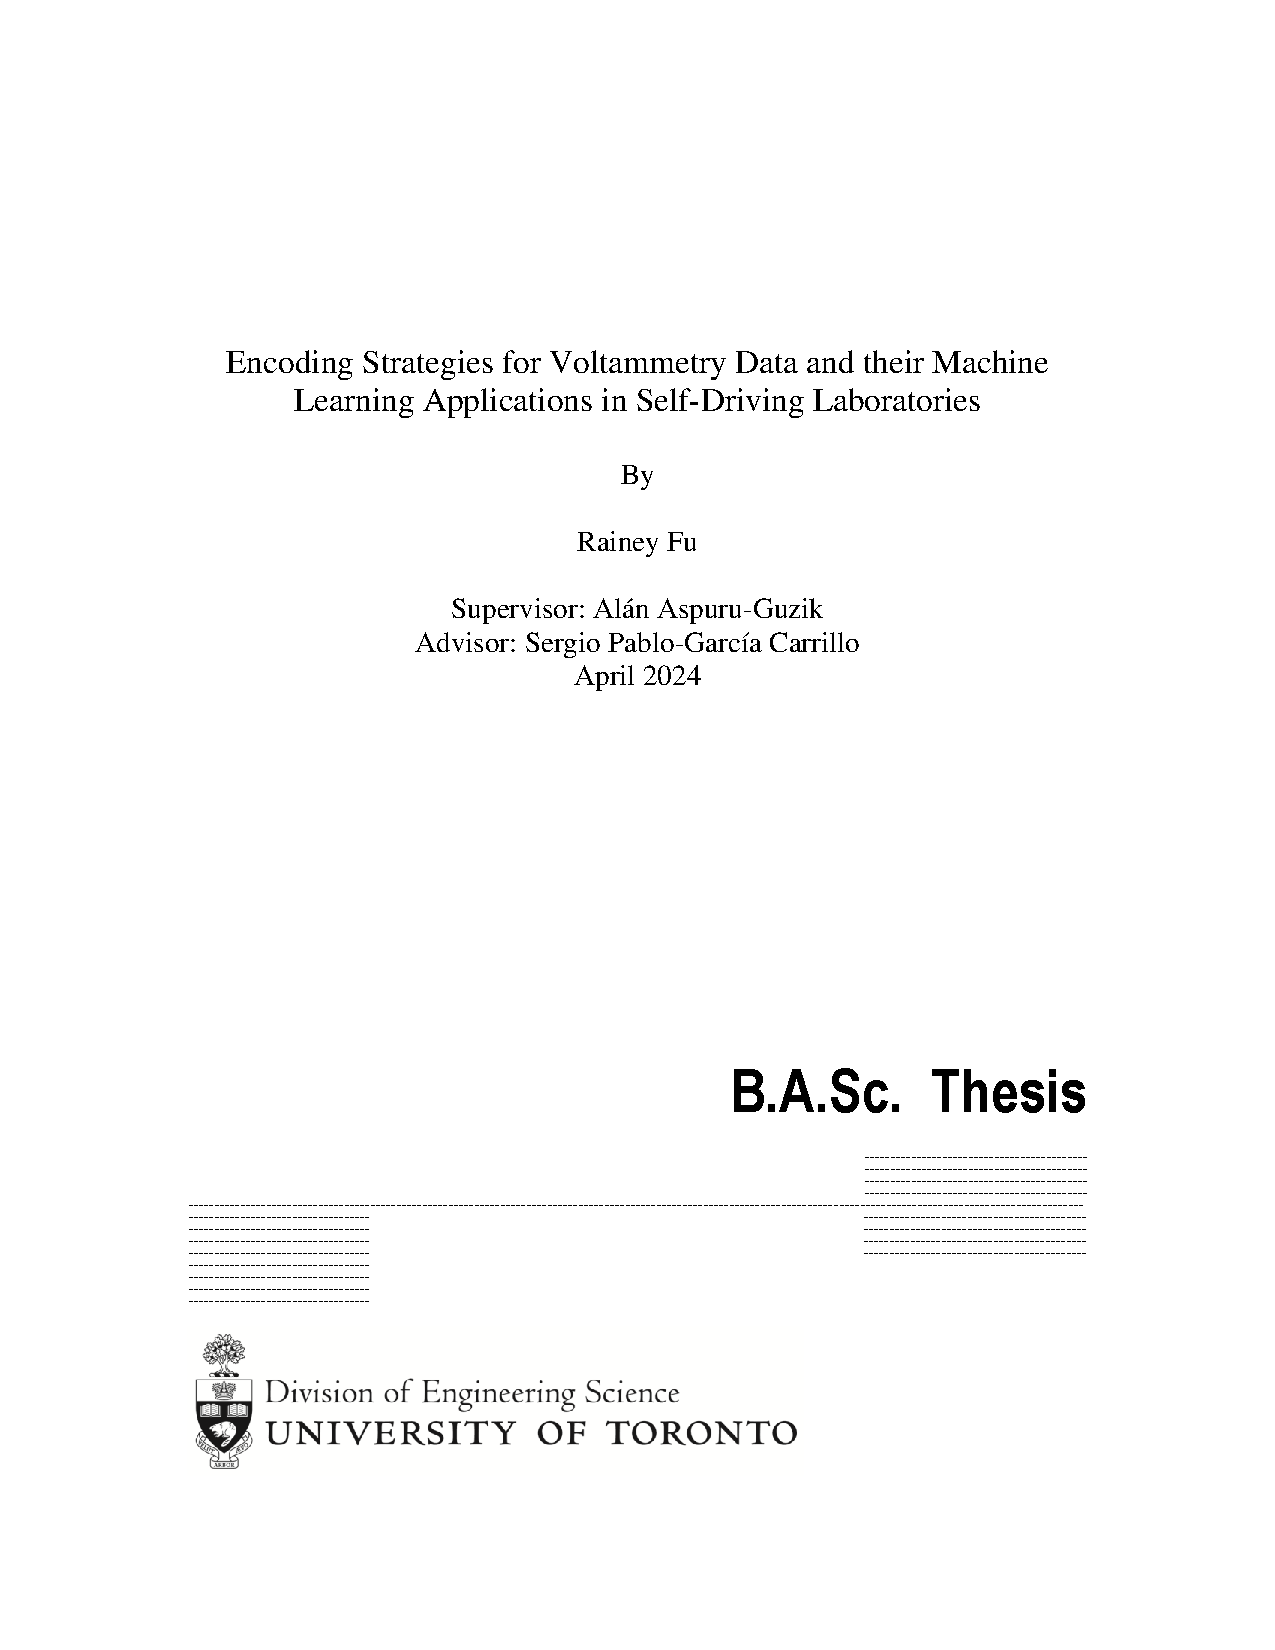
\includepdf[pages=-,width=\paperwidth]{title.pdf}
\clearpage                          % includ the title page


%% chapter header and page numbering set up
%% header unnumbered chapters (to remove the headers, comment out the following lines)
\pagestyle{fancy}
\fancyhead[R]{}                             % empty top-right header throughout the document
\fancyhead[L]{\nouppercase \leftmark}       % avoiding upper-case in header
\pagenumbering{roman}                       % pagination style: roman numeral
\setcounter{page}{2}                        % page counter starts at roman ii
\MainTextSpacing                            % double spacing for the contents


%% add abstract, dedication, and acknowledgment (and any other front matter)
\chap{Abstract} 

asdfasdf


%%  committee members go here (do not go to a new page; it should follow the abstract)
\begin{singlespace}

\textbf{Primary reader and thesis advisor:}

\vspace{0.2in}

\textbf{Secondary readers: }


\vspace{0.1in}

\end{singlespace}

%% single spacing is too cluttered and double spacing is too wide-spread
\TOCTextSpacing                             % one-half spacing for the table of contents
\renewcommand{\contentsname}{Table of Contents}
\tableofcontents
\listoftables
\addcontentsline{toc}{chapter}{List of Tables}
\listoffigures
\addcontentsline{toc}{chapter}{List of Figures}

%%%%%%%%%%%%%%%%%%%%%%%%%%% END FRONT MATTER %%%%%%%%%%%%%%%%%%%%%%%%%%%%





%%%%%%%%%%%%%%%%%%%%%%%%%%%%%% MAIN TEXT %%%%%%%%%%%%%%%%%%%%%%%%%%%%%%%%

\clearpage                                  % flushes the floats and new page
\pagenumbering{arabic}                      % arabic page numbering
\MainTextSpacing                            % restores double spacing in chapter contents

%% full header for the numbered chapters (to remove header comment out the following lines)
\renewcommand{\chaptermark}[1]{\markboth{#1}{#1}}
\fancyhead[L]{\chaptername\ \thechapter. \nouppercase \leftmark}


%% include all the main text chapters
\chapter{Background and Motivation} \label{chap:chap-1}

% if you want a short header you can use the following command
% \chapter[short-header-name]{chapter-title} \label{chap:chap-1}


% add your chapter text here
\section{Electrochemistry}
Given the pivotal role of reduction-oxidation (redox) reactions in materials chemistry and industrial applications, electrochemistry stands as a primary beneficiary of advancements in SDLs. According to the broad definition commonly accepted among researchers, electrochemistry encompasses the study of both the physical and chemical characteristics of ionic conductors, along with phenomena taking place at the interfaces between these ionic conductors and electronic conductors, semiconductors, other ionic conductors, and even insulating materials (such as gases and vacuum) \cite{Bagotsky2005}. The flow of electrons only occurs between two species, but the transfer of charge can also occur through an oxidation-reduction reaction. When a substance loses an electron, its oxidation state increases, indicating oxidation. When a substance acquires an electron, its oxidation state decreases, indicating reduction. For example, consider the following redox reaction, which has oxidation and reduction components:
\begin{align}
H\textsubscript{2} + F\textsubscript{2} \to 2HF \label{eq:reaction} \\
H\textsubscript{2} \to 2H\textsuperscript{+} + 2e\textsuperscript{-} \quad \text{Oxidation} \label{eq:oxidation}\\
F\textsubscript{2} + 2e\textsuperscript{-} \to 2F\textsuperscript{-} \quad 
\text{Reduction} \label{eq:reduction}
\end{align}
A redox reaction is balanced when the number of electrons gained by the oxidant is equal to the number of electrons lost by the reductant. Like any balanced chemical equation, the entire process is electrically neutral, meaning that the net charge remains consistent on both sides of the equation.
With redox reactions, it is possible to separate the oxidation \ref{eq:oxidation} and reduction \ref{eq:reduction} half-reactions physically in space, provided a complete circuit exists using an external electrical link, such as a wire, connecting the two halves. Electrons migrate from the reductant to the oxidant as the reaction progresses through this electrical connection, generating an electric current. 

Electrochemical cells are devices use redox reactions to generate electricity or use electricity to drive non-spontaneous redox reactions. This device effectively transforms chemical energy into electrical energy or vice-versa. In an electrochemical cell, reduction and oxidation reactions occur at the electrodes. The electrode where reduction occurs is termed the cathode, while oxidation occurs at the anode. An electrode serves as a stable electrical conductor, facilitating the flow of electrical current within non-metallic solids, liquids, gases, plasmas, or even vacuums. Electrodes are typically fabricated from highly conductive materials, including but not limited to metals and graphite \cite{goldbook}. In a battery, redox reactions create a flow of electrical current that can be used to power electronic devices.

Electrode potential is the voltage of an electrochemical cell composed of a reference electrode and another electrode to be characterized.
\begin{figure}[h!]
  \centering
    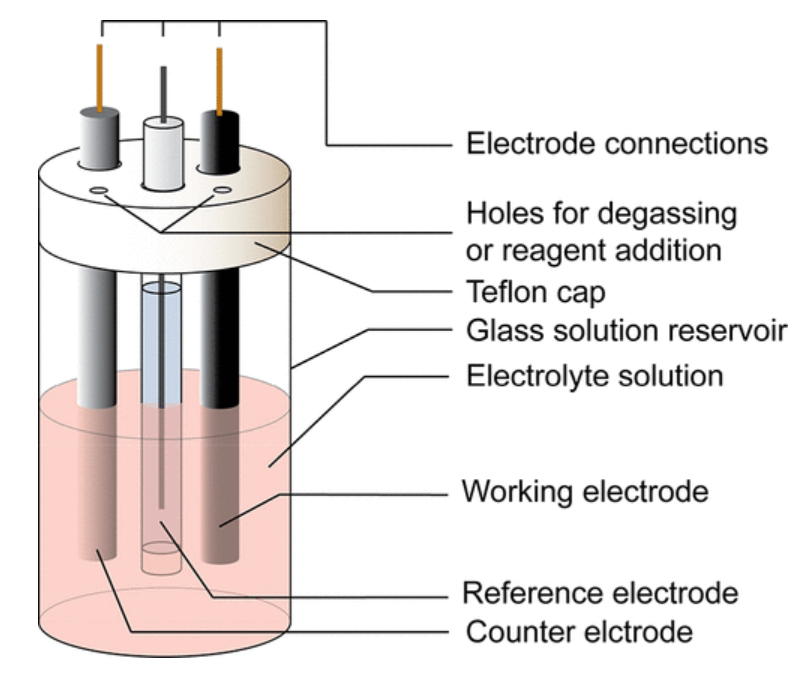
\includegraphics[width=0.8\textwidth]{figures/cv_diagram.png}
    \caption{Schematic of Electrochemical Cell \cite{Elgrishi2018}}
    \label{cell_schematic}
\end{figure}
Figure \ref{cell_schematic} shows a three-electrode setup typical for electrochemical experiments such as cyclic voltammetry. During the flow of current between the working and counter electrodes, the reference electrode is used to precisely measure the applied potential in relation to a stable reference reaction.
\begin{figure}[h!]
  \centering
    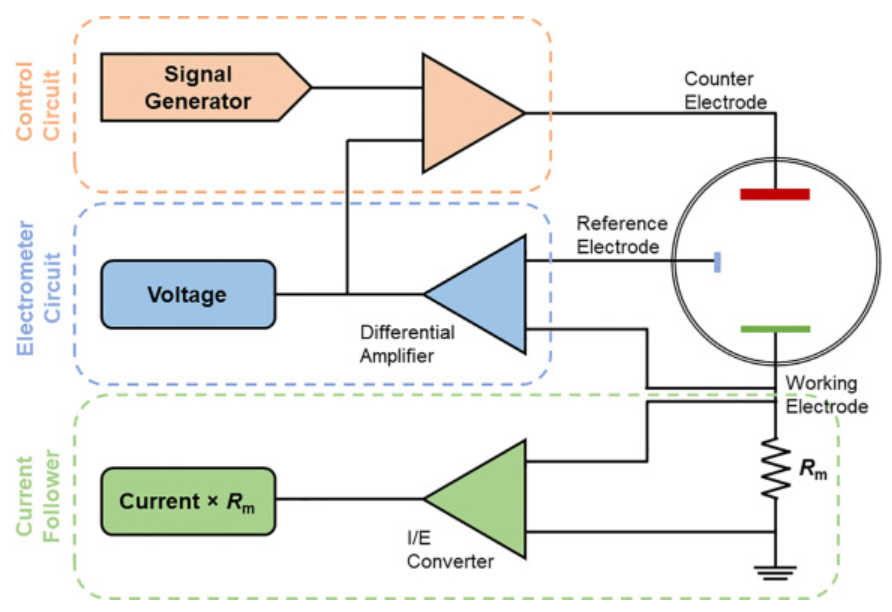
\includegraphics[width=1.0\textwidth]{figures/potentiostat_diagram.png}
    \caption{Potentiostat Circuit Diagram}
    \label{potentiostat_diagram}
\end{figure}
A potentiostat, as shown in Figure \ref{potentiostat_diagram}, is an analytical instrument designed to control the potential between the working electrode and counter electrode within a multi-electrode cell \cite{Zoski2006-zx}. The potentiostat contains various internal circuits tailored to fulfil this role, facilitating the generation and measurement of potentials and currents. External wires within a cell cable establish connections between the potentiostat circuit and the electrodes within the electrochemical cell. In a three-electrode configuration, the cell cable links the working, counter, and reference electrodes on one terminal and the potentiostat cell cable connector on the opposite end. The potentiostat's internal circuitry governs the applied signal. 

The working electrode performs the electrochemical event of interest. Since reactions occur at the cathode and anode surfaces, it is crucial that the surface is spotless and that the surface area is well-defined. The working electrodes should be immediately polished after use to ensure there are no surface contaminants that inhibit electron transfer. Even a few hours of air exposure will degrade the electrode surface. Detecting when surface contamination affects data quality is one of the questions this work addresses. This detection can trigger automatic polishing or replacement with a new disposable electrode \cite{Yoshikawa2024}.

Commercial vendors commonly provide potentiostats that are governed by proprietary software, employ graphical user interfaces (GUI), and produce already curated data. These devices are widely used for electroanalytical experiments such as cyclic voltammetry and differential pulse voltammetry. Commercial potentiostats can vary in design, but a typical potentiostat is shown in Figure \ref{potentiostat_diagram} and consists of three component circuits: a control circuit, an electrometer, and a current follower \cite{WAIN20211}. The electrometer circuit utilizes a differential amplifier to measure the difference in potential between the working and reference electrodes. Subsequently, the measured potential feeds into the control circuit, which administers a current through the counter electrode, altering the relative potential of the working electrode to align with the user-defined parameters. A single generator ensures this potential adheres to a predefined periodic waveform. The current flowing through the working electrode is then assessed by a current follower circuit, commonly in the form of a current-to-voltage converter. This circuit measures the drop in potential across a grounded resistor, allowing the current to be determined using Ohm's law.

However, commercial potentiostats present challenges for integration into automated systems due to their reliance on proprietary software and GUIs. Furthermore, their high cost poses a significant barrier for groups seeking to perform high-throughput analysis. To address these issues, Pablo-García et al. recently introduced an open-source, low-cost potentiostat \cite{PabloGarca2024}. Coupled with the synthesis platform reported in the same work, this innovative device aims to democratize electrochemical analysis by reducing the financial barrier to entry and improving integration with automation systems. By providing an affordable and accessible alternative to traditional commercial potentiostats, this open-source solution empowers researchers to conduct electrochemical experiments with greater flexibility and efficiency. Despite its remarkable advancements, the device's precision falls short of commercial standards. As such, we later explore various machine-learning methodologies to enhance data quality. 
\section{Cyclic Voltammetry}
\begin{figure}[h!]
  \centering
    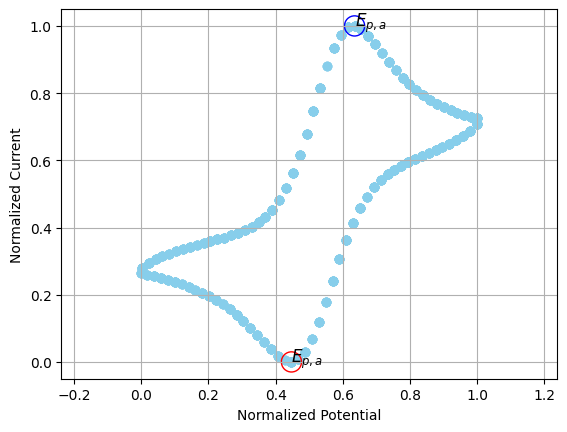
\includegraphics[width=1.0\textwidth]{figures/cv_example.png}
    \caption{Cyclic Voltammogram}
    \label{cv_example}
\end{figure}
Cyclic voltammetry (CV) is a common electrochemical characterization technique that extracts important redox information about molecules \cite{doi:10.1021/ac60210a007}. Typically, the working electrode potential increases linearly with time. After reaching a predetermined limit, the potential decreases to return to the starting voltage. These cycles can be repeated as frequently as needed to bolster confidence in the obtained data. The rate of voltage change over time is known as the experiment's scan rate \mbox{(Voltage/Time)} and affects how many data points are gathered throughout the experiment \cite{https://doi.org/10.1002/anie.198408313}. 

CV is valuable for studying qualitative information about electrochemical processes across diverse conditions. It enables the examination of intermediates in oxidation-reduction reactions and the assessment of reaction reversibility. Other use cases include the determination of electron stoichiometry, analyte diffusion coefficients, and formal reduction potentials, aiding in identification processes \cite{Nicholson1964}. Additionally, in reversible Nernstian systems, the proportional relationship between concentration and current allows for determining unknown solution concentrations by constructing calibration curves correlating current and concentration \cite{Libretexts_2023}.

In a typical cyclic voltammogram shown in Figure \ref{cv_example}, peaks represent electrochemical processes occurring at the electrode surface. The anodic peak ($\mathrm{E_{p, a}}$) is observed during the scan where oxidation of the electroactive species occurs at the electrode and corresponds to the potential at which oxidation is most favourable. The current increases as the potential applied to the electrode becomes more positive, reaching a maximum at the peak potential. The cathodic peak ($\mathrm{E_{p, c}}$) is observed during the reverse scan where reduction of the electroactive species occurs at the working electrode and corresponds to the potential at which reduction is most favorable. The current increases as the potential becomes more negative, reaching a maximum at the peak potential \cite{GRIMSHAW20001}. Typically, chemists are especially interested in these peaks as they condense the redox behavior of the analyzed compound \cite{Faulkner1983}.
\section{Differential Pulse Voltammetry}
\begin{figure}[h!]
  \centering
    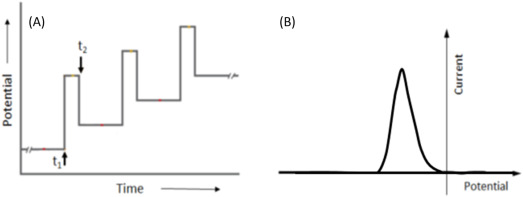
\includegraphics[width=1.0\textwidth]{figures/dpv.jpg}
    \caption{Differential Pulse Voltammogram}
    \label{dpv_example}
\end{figure}
Differential Pulse Voltammetry (DPV) is a more sophisticated electrochemical measurement technique where a series of increasing pulses are applied across the electrodes in an electrochemical cell \cite{Scholz2005-pa}. The current $I_1$ is measured right before applying the pulse at time $t_1$, and $I_2$ is measured again at the end at time $t_2$. The difference in current $\Delta I(I_2 - I_1$) is plotted against the potential and results in a peak-like shape. 
This method helps reduce the impact of charging current by sampling the current just before the potential change. DPV is well suited for measurements with extremely low concentrations of chemicals. This is because the effect of the charging current can be minimized to achieve high sensitivity, and only the faradaic current, the electric current generated by the redox of a chemical at an electrode, is extracted so that electrode reactions can be measured precisely \cite{Laborda2014}. Furthermore, DPV is a versatile tool for the qualitatively characterizing chemical compounds and their electrochemical properties \cite{Scholz2005-pa}. By analyzing the shape, position, and area of the peaks in the DPV curve, chemists can glean insights into the nature of the electroactive species present, their concentration, kinetics of electron transfer processes, and other relevant electrochemical parameters. This capability makes DPV invaluable in various fields such as analytical chemistry, environmental monitoring, and pharmaceutical research, where understanding the behaviour of chemical compounds at the molecular level is crucial \cite{Scholz2005-pa}.
\chapter{Clustering} \label{chap:chap-2}

% if you want a short header you can use the following command
% \chapter[short-header-name]{chapter-title} \label{chap:chap-2}


% if you want to add the quote above the chapter heading then do the following:
% (for this case, you may have to change \ChapterTopSpace in the main file)
% \epigraphhead[0]{whole-above-epigraph-goes-here}


% add the citation for the chapter if it is a reprint


% add your chapter text here
\section{Introduction}
Given the capabilities and limitations of SDLs, there exists a need for a quick and accurate characterization of the produced electrical compounds. Clustering experimental results becomes crucial for several reasons. 
Clustering identifies patterns and similarities among experimental results. This aids in the discovery of underlying trends or relationships between different compounds or experimental conditions. It also facilitates quality control by pinpointing outliers or anomalies in experimental data, ensuring the reliability of data produced by SDLs. 
Moreover, clustering allows researchers to optimize processes by providing insights into the effects of various parameters on the formation of electrical compounds. This optimization can significantly enhance the efficiency of the voltammetry process in SDLs. Additionally, by classifying different types of electrical compounds based on their properties or characteristics, clustering supports classification and prediction tasks, enabling researchers to predict the behavior of new compounds or classify unknown compounds based on their similarities to known clusters.
Finally, clustering provides a structured way to organize and interpret large volumes of experimental data, facilitating decision-making processes related to the selection of compounds for further analysis or the design of future experiments. In essence, clustering experimental results in the context of SDLs used for voltammetry is indispensable for gaining insights, ensuring data quality, optimizing processes, classifying compounds, and facilitating decision-making processes.
\section{Data Collection}
To analyze how data gathered from SDLs can be clustered, data was gathered through a cost-effective autonomous electrochemistry experimentation that operates through an iterative workflow \cite{PabloGarca2024}. The workflow was used to synthesize and characterize 10 distinct metals and 10 distinct ligands, with specific details available in Appendix \ref{metal_table} and Appendix \ref{ligand_table}, resulting in 100 unique complexes. Each complex was synthesized using a metal/ligand concentration ratio of 1:7 to ensure complete complexation. The synthesis process employed 1.0 M NaCl in water as the electrolyte/solvent, and a buffer solution consisting of a 1:1 ratio of HOAc/NaOAc. Following synthesis, comprehensive characterizations were conducted using cyclic voltammetry (CV) and differential pulse voltammetry (DPV) techniques. The experimentation was done using a low-cost electrochemistry platform designed as an alternative to commercial options. The length of these samples may vary due to differing scan rates. Higher scan rates lead to more data points being collected during the experiment and can provide finer resolution of the electrochemical processes occurring. Additionally, it's worth noting that these samples may be duplicated as CV and DPV analyses can be conducted multiple times on the same sample. Importantly, the workflow is adaptable, with the potential to encompass a broader range of parameters, including additional ligands, varying metal/ligand ratios, mixed ligands, different buffer pH levels, and reaction times. The accumulation of data points is ongoing, contributing to the continuous expansion and refinement of our understanding. The final dataset consists of 800 CV data points and 200 DPV data points. The dataset used in this work can be found in the article preprint \cite{PabloGarca2024}.
\section{Curse of Dimensionality}
The curse of dimensionality refers to the phenomena that cause various challenges and complications when analyzing data in high-dimensional spaces. As the number of features in a dataset increases, the amount of data needed to generalize accurately grows exponentially. As the number of dimensions increases, the data becomes increasingly sparse. This makes tasks like clustering and classification more challenging. In higher dimensions, the difference between distances between data points starts to become negligible, making measurements like Euclidean distance negligible. As such, algorithms that rely on distance measurements will experience a drop in performance. Furthermore, more dimensions will require more computational resources and time to process the data. It is good practice to aim to have the data in as low-dimension as possible provided relevant information is maintained. 
\section{K-Means}
\begin{figure}[h!]
  \centering
    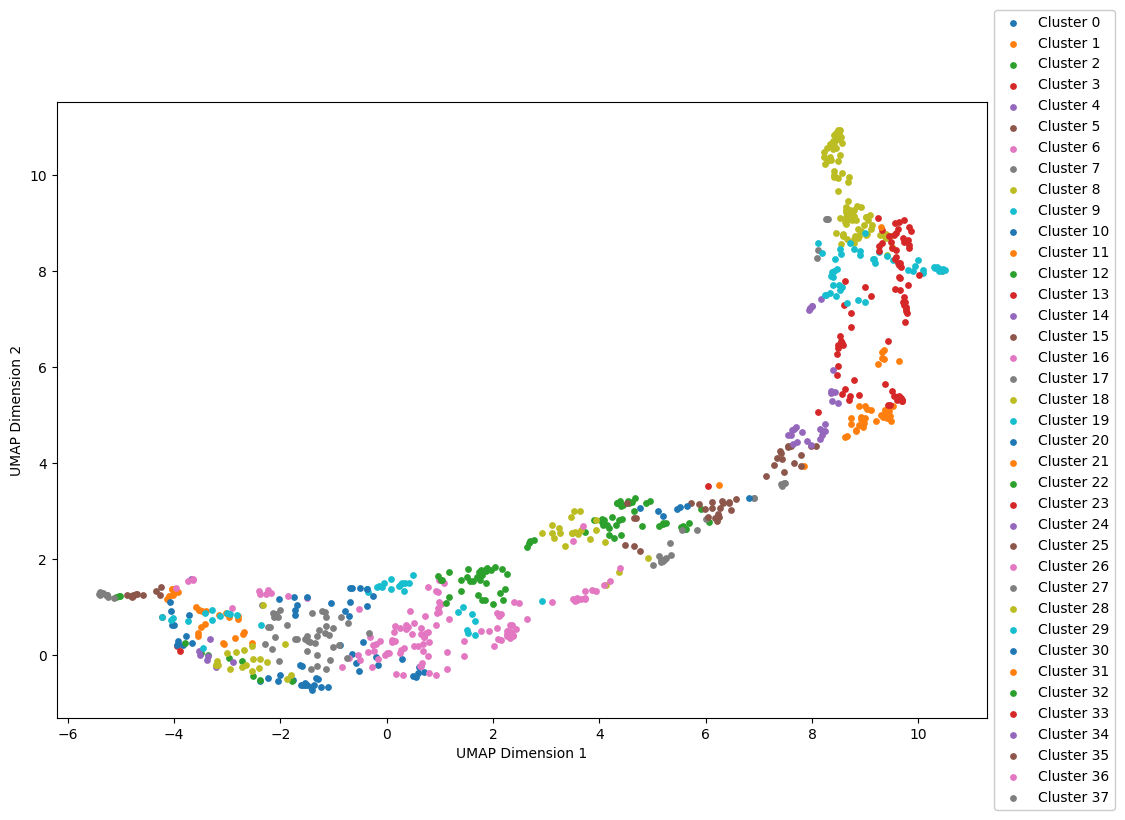
\includegraphics[width=1.0\textwidth]{figures/k-means.png}
    \caption{CV K-Means Clustering Visualized}
    \label{kmeans}
\end{figure}
K-Means clustering is an unsupervised machine learning algorithm aimed to divide a set of data points into clusters such that the data points within each cluster are similar and different from the data points in other clusters \cite{MacQueen1967}. The K-Means clustering result for CV data can be seen in Figure \ref{kmeans}. The algorithm is explained below with K representing the desired number of clusters:
\begin{enumerate}
    \item Initially, K points are selected randomly as the cluster centroids
    \item Each data point is assigned to the closest mean, quantified by the Euclidean distance. 
    \item Each cluster centroid is updated to reflect the average of data points currently assigned to that cluster 
    \item This process is repeated for a specified number of iterations
\end{enumerate}
One of the questions that needs to be answered is the choice of K. This means finding a balance between the number of clusters represented by K and the average variance of the clusters while minimizing both. There is no approach for determining K that works better than all others in all cases. For this problem of clustering CV and DPV data, a combination of the Elbow Method and Silhouette method is used. The Elbow Method is done by plotting the within-cluster sum of squares (WCSS) for a range of K and choosing the value K where adding more clusters does not significantly decrease the WCSS. While the Elbow Method can easily eliminate many values of K, it also has drawbacks regarding the shape of the WSCC curve. Determining the exact location of the "elbow" can be subjective and depends on the analyst's interpretation. Different individuals may identify different elbows, leading to inconsistency in results. In cases where the relationship between the number of clusters and WCSS is not distinctly elbow-shaped, the Elbow Method may not provide clear guidance for choosing the appropriate number of clusters. The Silhouette Method addresses some of these drawbacks by providing a more quantitative measure of cluster quality. Instead of relying on subjective interpretation, the Silhouette Method calculates the silhouette coefficient for each data point, which quantifies how similar an object is to its own cluster compared to other clusters. This provides a more objective measure of cluster cohesion and separation. The process for selecting K for this work includes determining a set of candidate K values using the Elbow Method by eliminating obviously suboptimal values and then using the Silhouette method to find optimal K among the potential candidates. 
\section{Density-Based Spatial Clustering of Applications with Noise}
\begin{figure}[h!]
  \centering
    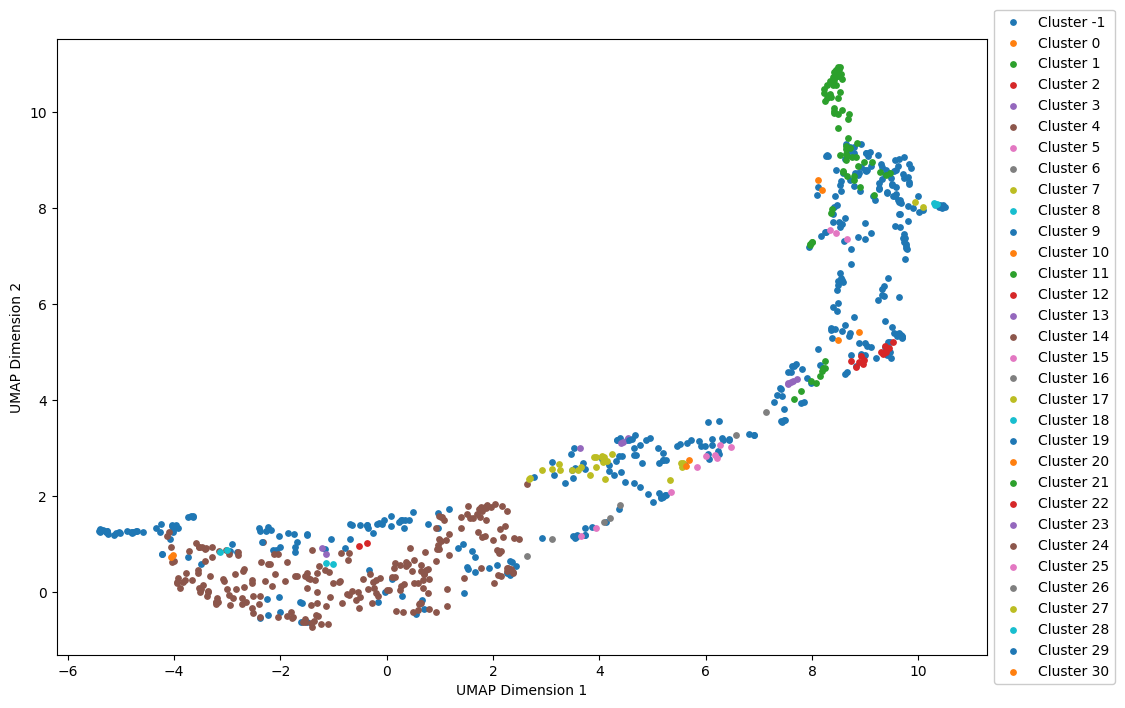
\includegraphics[width=1.0\textwidth]{figures/dbscan.png}
    \caption{CV DBSCAN Clustering Visualized}
    \label{dbscan}
\end{figure}
Density-Based Spatial Clustering of Applications with Noise (DBSCAN) is another clustering algorithm that works by partitioning the data into dense regions of points that are separated by less dense areas \cite{Ester1996ADA}. It defines clusters as areas of the dataset where there are many points close to each other, while the points that are far from any cluster are considered outliers or noise. In DBSCAN, eps ($\epsilon$) represents the maximum distance between two points for them to be considered neighbours, and minimum samples is the number of points required for a point to be considered a core point. Points that have fewer than minimum samples points are labelled as noise. The key differentiator for DBSCAN is that the number of clusters does not need to be determined beforehand.  
\section{t-Distributed Stochastic Neighbor Embedding}
Dimensionality techniques like t-Distributed Stochastic Neighbor Embedding (t-SNE) are used for visualizing high-dimensional data in a low-dimensional space \cite{vanDerMaaten2008}. This visualization can aid in the clustering process by providing insights into the underlying structure of the data and help in understanding the results of the clustering algorithm. The first step of the algorithm is to create a probability distribution that represents the similarity between neighbors. The similarity between the two data points is represented by their Euclidean distance. For each data point, it is placed in the middle of the Gaussian curve and the rest of the data is placed along the curve. This is represented by the following equation where $j \neq i$ and $p_{i|i} = 1$:
\begin{align}
p_{j|i} = \frac{exp(-||x_i - x_j||^2 / 2\sigma_i^2)}{\sum_{k \neq i}exp(-||x_i - x_k||^2 / 2\sigma_i^2)}
\end{align}
"The similarity of datapoint $x_j$ to datapoint $x_i$ is the conditional probability, $p_{j|i}$, that $x_i$ would pick $x_j$ if neighbors were picked in proportion to their probability density under a Gaussian centered at $x_i$" \cite{vanDerMaaten2008}. The last variable that has not been discussed yet is sigma. This variable is not chosen directly, but rather by choosing a value for perplexity. Perplexity is defined as:
\begin{align}
Perp(p) \coloneq 2^{-\sum_x p(x)log_2(p(x))}
\end{align}
Perplexity represents the density of data and how many neighbors the central point should have with higher values relating to higher variance. After choosing the perplexity value, the corresponding sigma values are found using binary search. 
Next, the similarities between data points for low-dimensional representational will also need to be found to ensure that similar data are close together after projection. 
\section{UMAP}
Uniform Manifold Approximation and Projection (UMAP) is a dimension reduction technique that can be used for visualization similarly to t-SNE \cite{https://doi.org/10.48550/arxiv.1802.03426}. It achieves this by leveraging concepts from algebraic topology and Riemannian geometry.
Here's a simplified breakdown of how UMAP works:
\begin{enumerate}
\item Constructing a Topological Representation: UMAP starts by creating a fuzzy topological representation of the data. This involves building a simplicial complex, which is a way to represent topological spaces using simple geometric shapes called simplices. The algorithm constructs these simplices based on the proximity of data points to each other.
\item Optimizing Low-Dimensional Representation: Once the topological representation is established, UMAP then optimizes a low-dimensional representation of the data to match this topological structure as closely as possible. It does this by minimizing a measure called cross-entropy, which quantifies the difference between the fuzzy topological structures of the high-dimensional and low-dimensional data.
\item Efficient Computations: UMAP employs several strategies to make computations efficient. It focuses on computing only the nearest neighbours of each point and uses algorithms like Nearest-Neighbor-Descent for this purpose. Additionally, it utilizes stochastic gradient descent for optimization and smooth approximations of the membership strength function to ensure differentiability.
\item Preserving Topological Structure: The goal of UMAP is to ensure that the low-dimensional representation maintains the essential topological properties of the original data. It achieves this by balancing attractive forces that pull similar points together and repulsive forces that push dissimilar points apart, based on the weights of edges in the topological representation.
\end{enumerate}
\section{Ramer–Douglas–Peucker Algorithm}
\begin{figure}[h!]
  \centering
    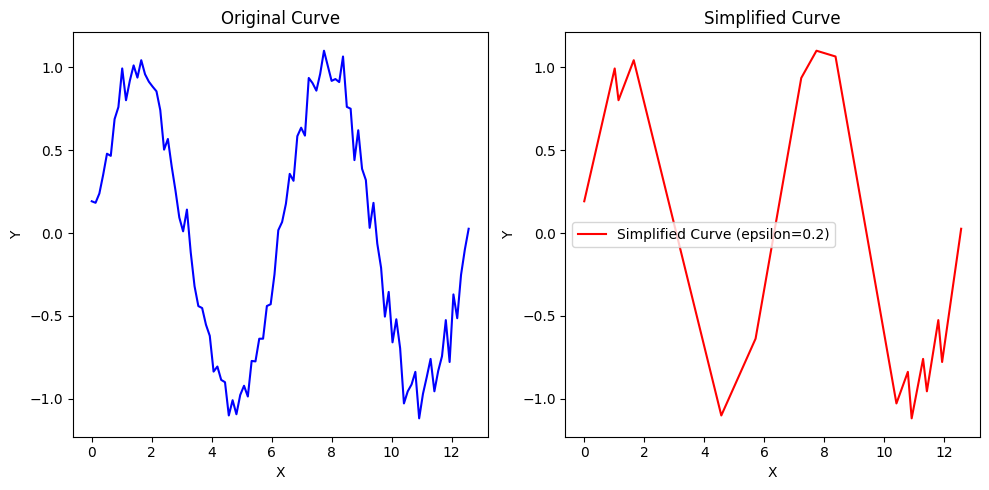
\includegraphics[width=1.0\textwidth]{figures/rdp.png}
    \caption{RDP Algorithm}
    \label{rdp}
\end{figure}
The Ramer–Douglas–Peucker (RDP) algorithm is employed to reduce the number of points in a curve approximated by a series of points. It operates by conceptualizing a line between the initial and terminal points within a point set defining the curve. Subsequently, it identifies the point furthest from this line among the intermediary points. If this point, termed the "outlier point", and consequently all intervening points, lie within a specified distance 'epsilon' from the line, they are removed. Conversely, if the outlier point surpasses the epsilon threshold, the curve is segmented into two parts: from the initial point to the outlier point, inclusive and the outlier point and the remaining points. The algorithm is then recursively applied to both resulting segments, and the reduced forms of the curve are reassembled. Since CV and DPV results can be represented as a curve, RDP can be used to remove unnecessary points while maintaining the overall shape of the voltammogram. This will reduce the dimensionality and improve data analysis results.
\section{Data Preparation and Encoding}
Many parameters can be set during CV and DPV analysis, affecting the outcomes of the characterization. Particularly, the experiment's scan rate affects the sampling frequency and the number of points collected within a certain time interval, leading to a variable number of point densities depending on the analyzed compound. Heterogeneity among samples becomes challenging for many ML algorithms, as they often require input data to be the same shape. Similarly, the potential limit at which the potential begins to return to its initial point will affect the overall shape of the cyclic voltammogram. To handle this, the following steps are used to prepare the data:
\begin{enumerate}
    \item Split experiment cycles into separate data points
    \item Normalize values to fit between [0, 1]
    \item Reduce points using the Ramer-Douglas-Peucker algorithm
    \item Duplicate data points until the total length reaches the longest cycle's length
    \item Order data points based on angular position relative to the center
\end{enumerate}
Due to the curse of dimensionality, the RDP algorithm is used to reduce the number of dimensions. Since the RDP algorithm takes only a variable $\epsilon$, the final length after reduction will be different for each set of data. To ensure the data has the same length as the longest data after RDP reduction, data points are randomly selected and duplicated. Finally, the data is ordered based on its angular position relative to the center for consistency.
\begin{figure}[h!]
  \centering
    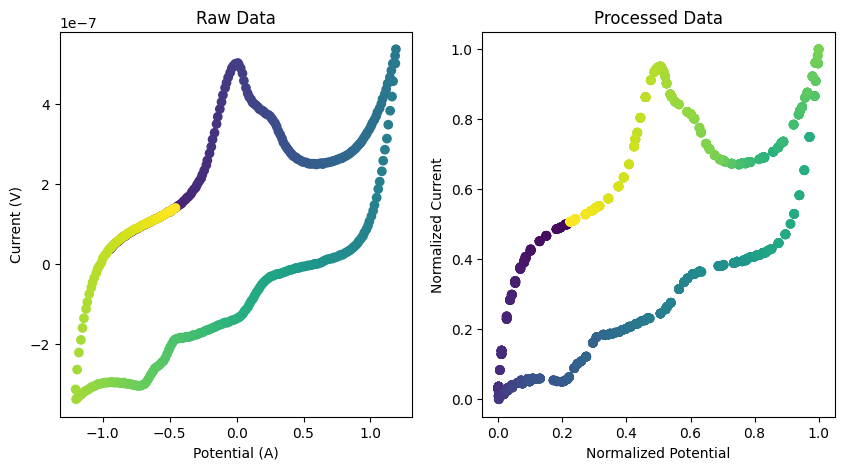
\includegraphics[width=1.0\textwidth]{figures/encoding.png}
    \caption{Raw Data and Processed Data}
    \label{encoding}
\end{figure}
Plots of the raw data and processed data can be seen in Figure \ref{encoding} with the color of the scatter plot representing the order in which the points appear. The starting point and end point varies across different voltammetry experiments. As such, it is important to order the data points so that comparisons can be informative. A significant reduction in dimensionality by 1/3 can also be seen in the plots. Despite this, the important characteristics of the voltammogram such as the overall shape and peaks are maintained.
\section{Results and Discussion}
To categorize the experimental data, the K-Means clustering algorithm was used post-processing the entire set of experimental voltammetry. With K-Means, a value of K will need to be selected. This is done using the elbow method. Figure \ref{elbow} shows the results of the elbow method applied to the dataset. It can be seen that this methodology identifies multiple potential candidates for K-values, necessitating a more comprehensive analysis to select the most appropriate option. 
\begin{figure}[h!]
  \centering
    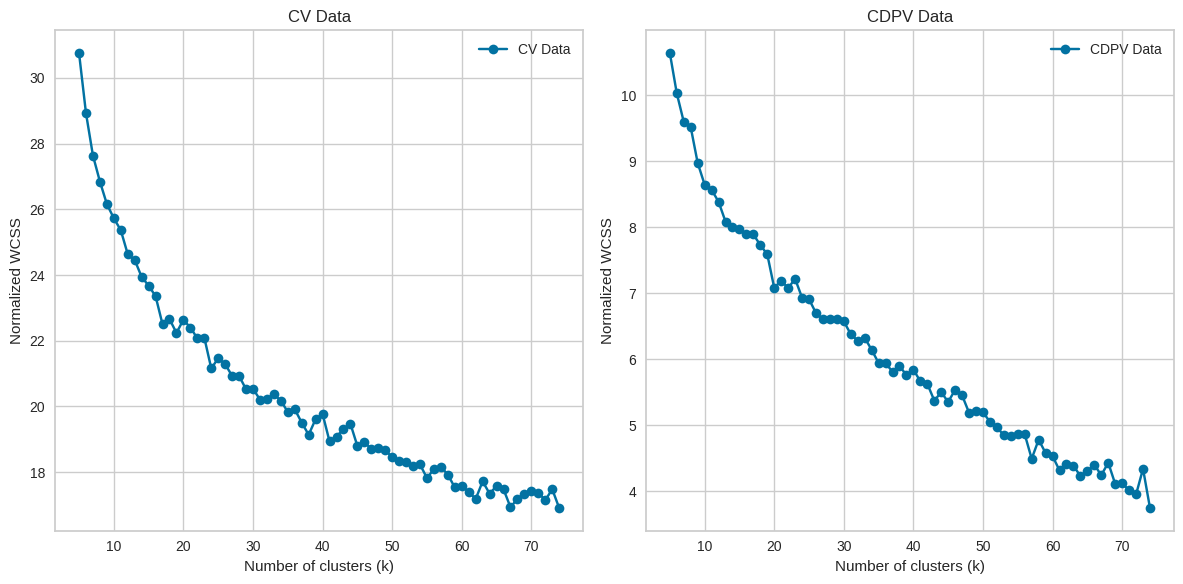
\includegraphics[width=1.0\textwidth]{figures/elbowmethod.png}
    \caption{K-Means Elbow Method}
    \label{elbow}
\end{figure}
To aid the decision-making process, the Silouhette method is used to analyze promising values \cite{ROUSSEEUW198753}. A cluster with a value of 1 means points are perfectly assigned in a cluster and clusters are easily distinguishable, 0 means clusters are overlapping, and -1 means points are assigned to the wrong cluster. The K value should be chosen based on which value produces the most clusters with Silhouette scores greater than the average score of the dataset, represented by the red-dotted line seen in Figure \ref{cv_silhouette} and Figure \ref{dpv_silhouette}. Furthermore, there should not be wide fluctuations in the size of the clusters. The width of the clusters represents the number of data points belonging to the cluster. 
\begin{figure}[h!]
  \centering
    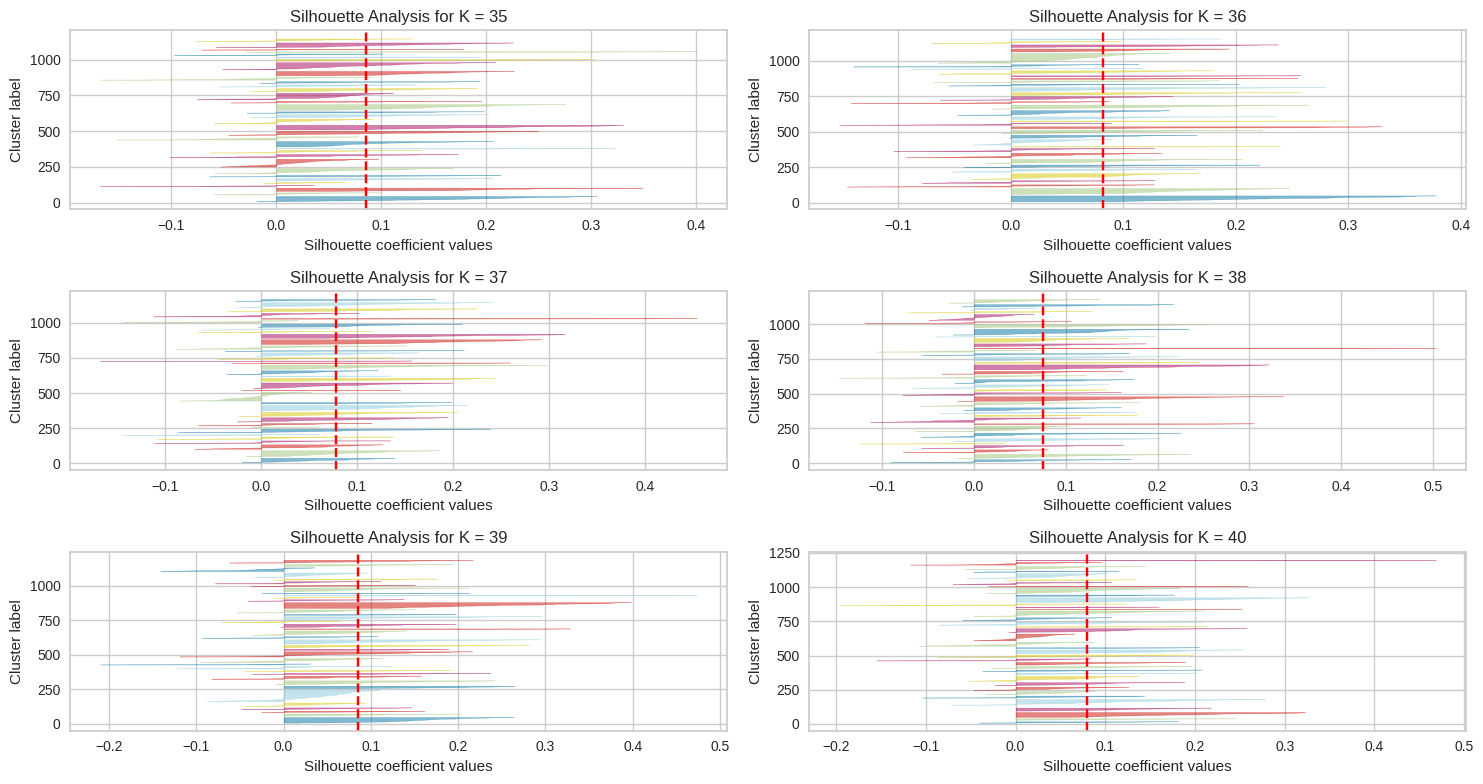
\includegraphics[width=1.0\textwidth]{figures/cv_silhouette.png}
    \caption{CV Silhouette Method}
    \label{cv_silhouette}
\end{figure}
In Figure \ref{cv_silhouette}, which showcases the application of the Silhouette method for CV cross-validation, K = 38 yields the highest number of clusters with a score surpassing the mean of the dataset. This configuration not only reduces the number of clusters scoring below zero but also minimizes the variance in cluster sizes.
\begin{figure}[h!]
  \centering
    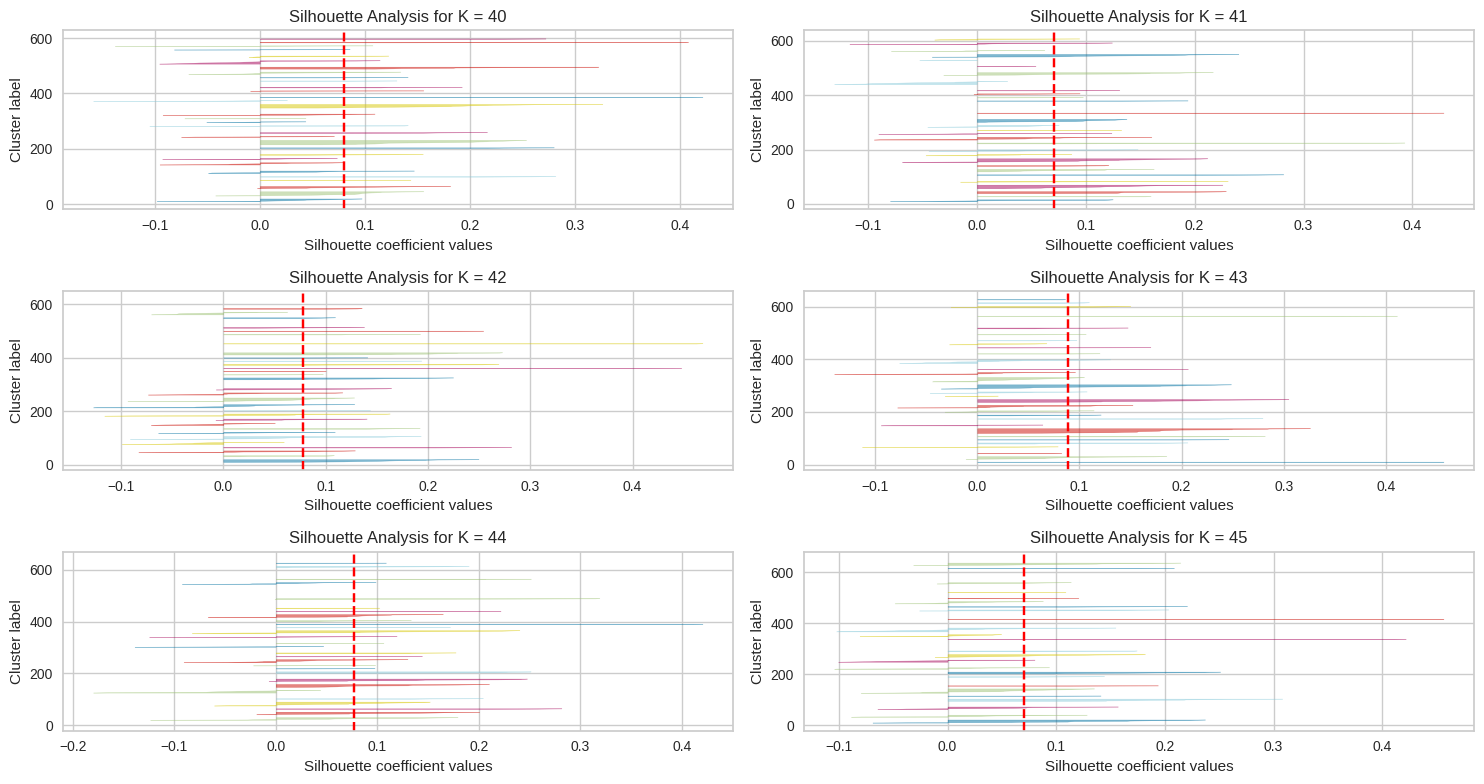
\includegraphics[width=1.0\textwidth]{figures/dpv_silhouette.png}
    \caption{DPV Silhouette Method}
    \label{dpv_silhouette}
\end{figure}
Similarly, in Figure \ref{dpv_silhouette} showcasing the Silhouette method for DPV, K = 42 results in the best quality of clusters. A subset of the cluster results is available in the appendix. Despite having 100 different combinations of metals and ligands, using a relatively small K value still shows promising results, as the data points within each cluster have similar overall shapes, which is crucial for compound identification. 

\begin{figure}[h!]
  \centering
    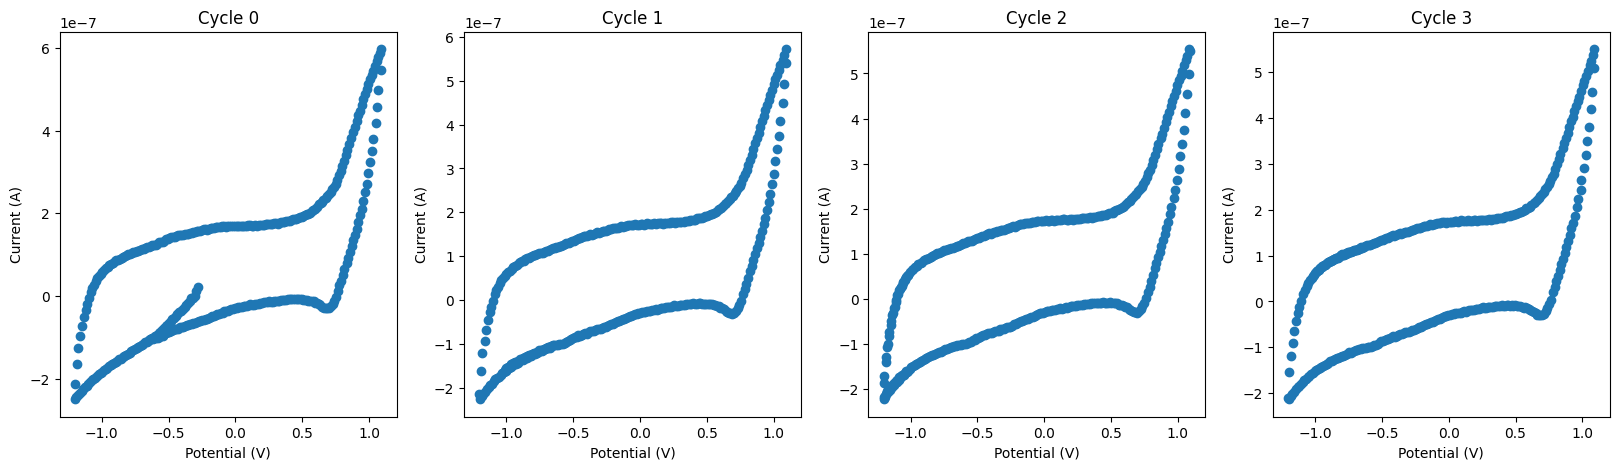
\includegraphics[width=1.0\textwidth]{figures/dbscan_results.png}
    \caption{DBSCAN Clusters}
    \label{dbscan_results}
\end{figure}
DBSCAN, as an alternative clustering method, demonstrated significant promise in identifying anomalous data points. With the appropriate parameters, DBSCAN efficiently grouped cycles originating from the same experiment. As depicted in Figure \ref{dbscan_results}, DBSCAN defines a cluster comprising cycles solely from a single experiment. This capability could be seamlessly incorporated into SDLs as an error validation mechanism. Any cycle not assigned to the same cluster as others from the identical experiment could trigger an error notification, prompting intervention and investigation.

To further demonstrate the efficacy of the encoding, t-SNE and UMAP projections are created to visualize the data in 2-D and show how the shapes, metals, and ligands are distributed. Interactive plots made with Bokeh are available on \href{https://github.com/raineyfu/Thesis}{Github}.
\begin{figure}[h!]
  \centering
    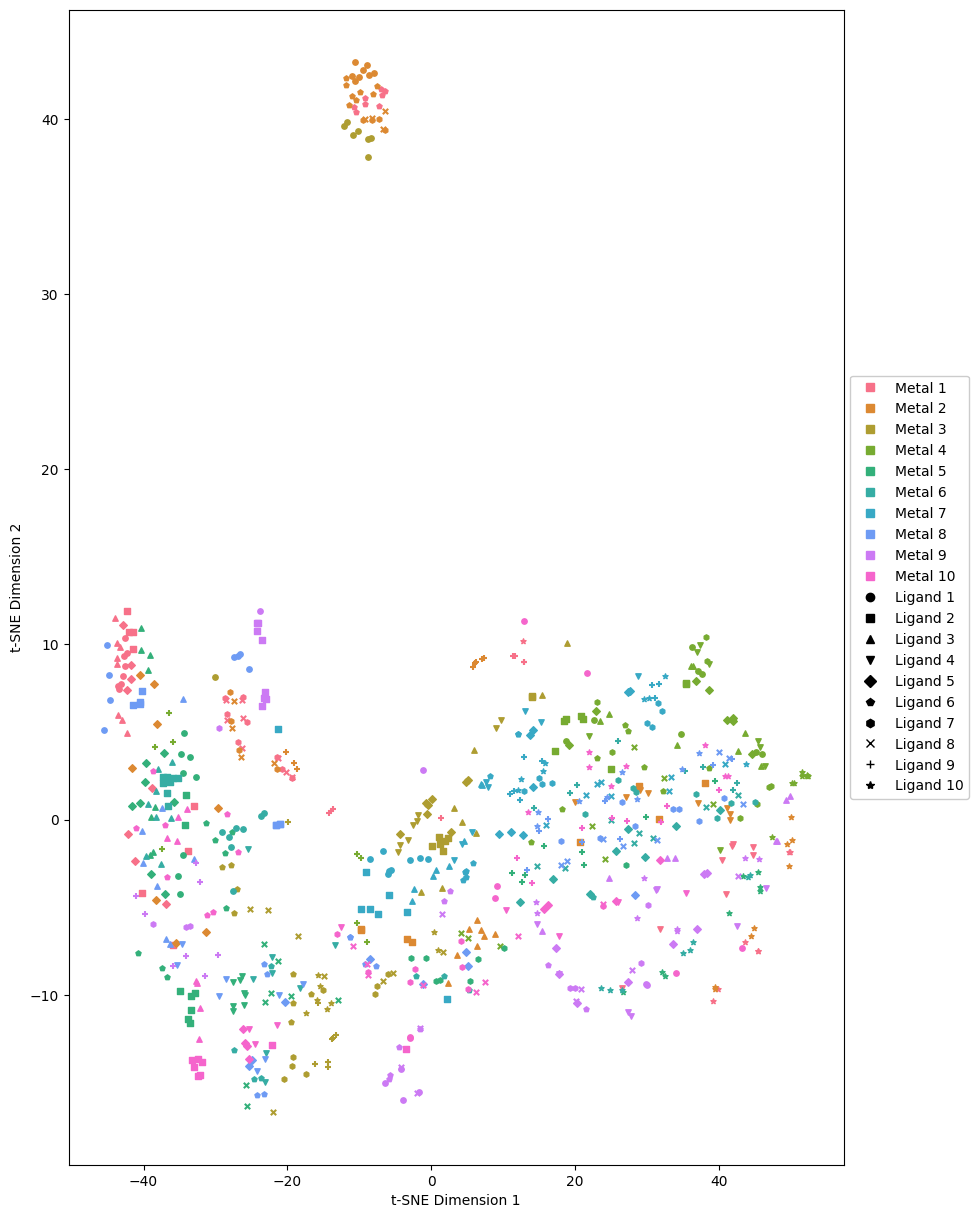
\includegraphics[width=1.0\textwidth]{figures/cv_tsne.png}
    \caption{Cyclic Voltammetry t-SNE Projection}
    \label{cv-tsne}
\end{figure}
\begin{figure}[h!]
  \centering
    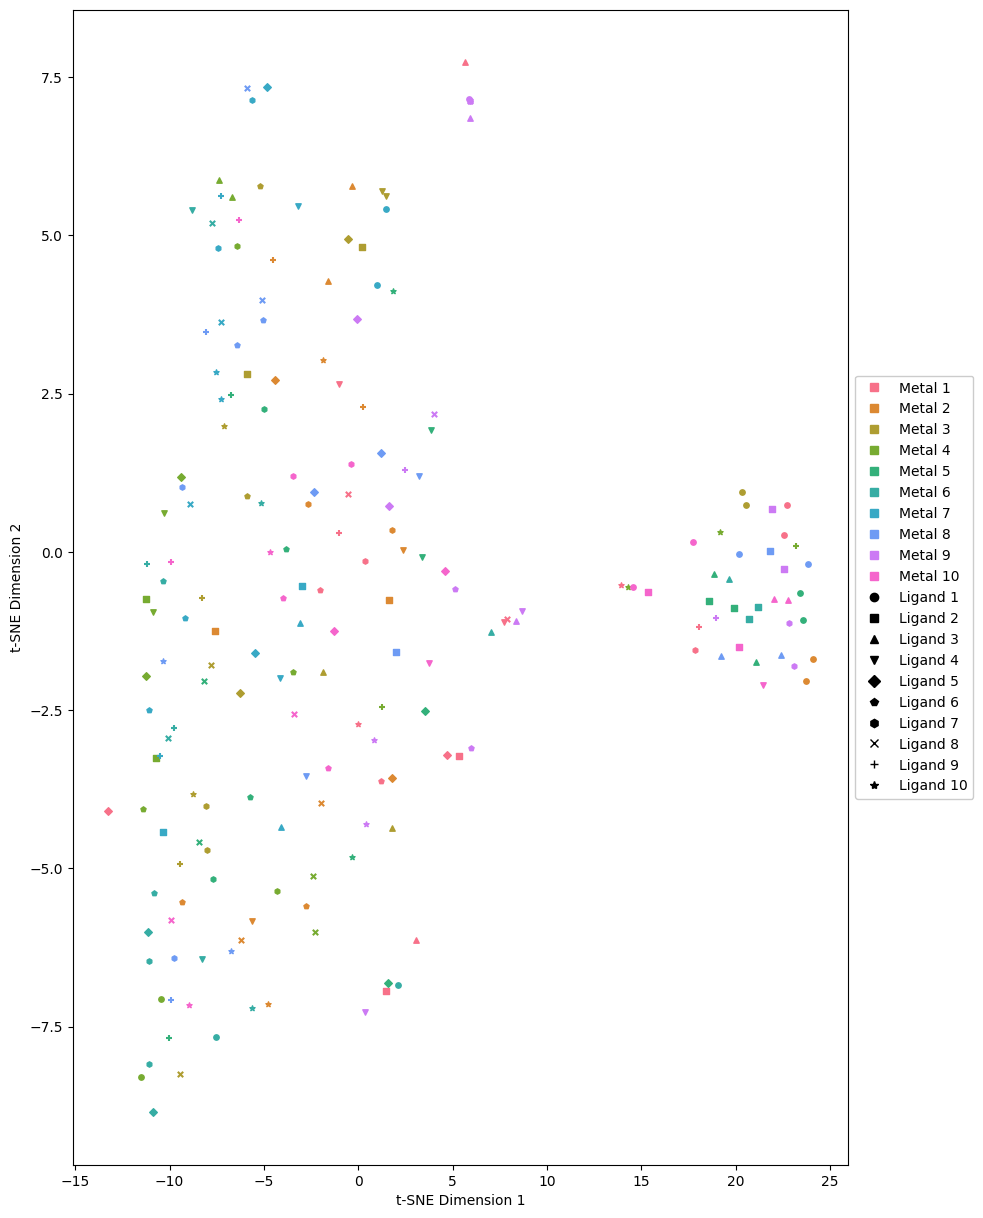
\includegraphics[width=1.0\textwidth]{figures/dpv_tsne.png}
    \caption{Differential Pulse Voltammetry t-SNE Projection}
    \label{dpv-tsne}
\end{figure}
As seen in Figure \ref{cv-tsne} and Figure \ref{dpv-tsne}, t-SNE emphasizes local structure and tends to agglomerate similar data points into tight clusters. As a result, t-SNE plots often show clearer separation between clusters but may not preserve the global structure as effectively. t-SNE primarily preserves local neighborhoods, which leads to tighter clusters of similar points. However, it may not always capture the global structure accurately, especially for complex datasets. t-SNE embeddings can vary significantly with different random initializations and parameter choices, making it less stable and potentially more sensitive to noise in the data. 
\begin{figure}[h!]
  \centering
    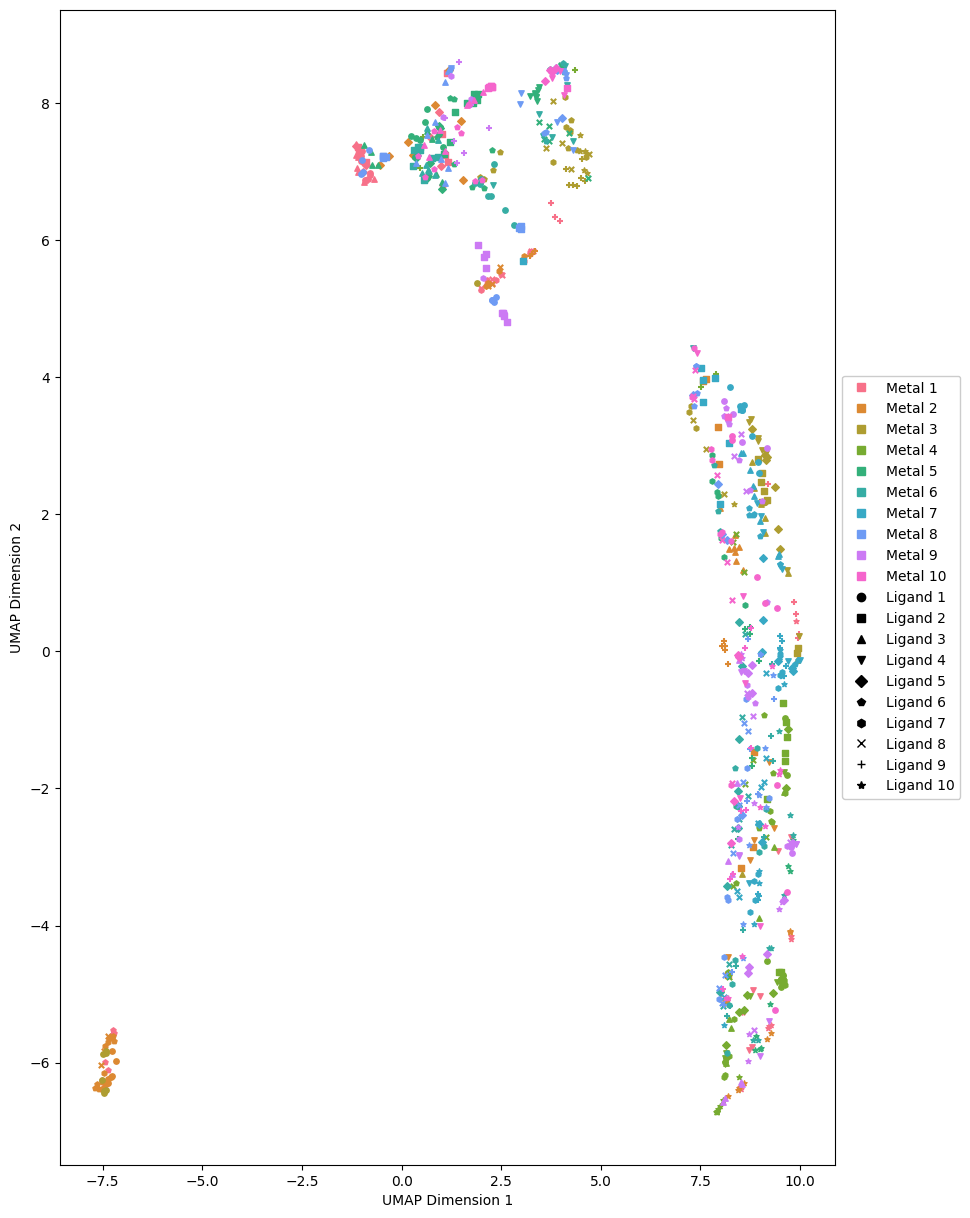
\includegraphics[width=1.0\textwidth]{figures/cv_umap.png}
    \caption{Cyclic Voltammetry UMAP Projection}
    \label{cv-umap}
\end{figure}
\begin{figure}[h!]
  \centering
    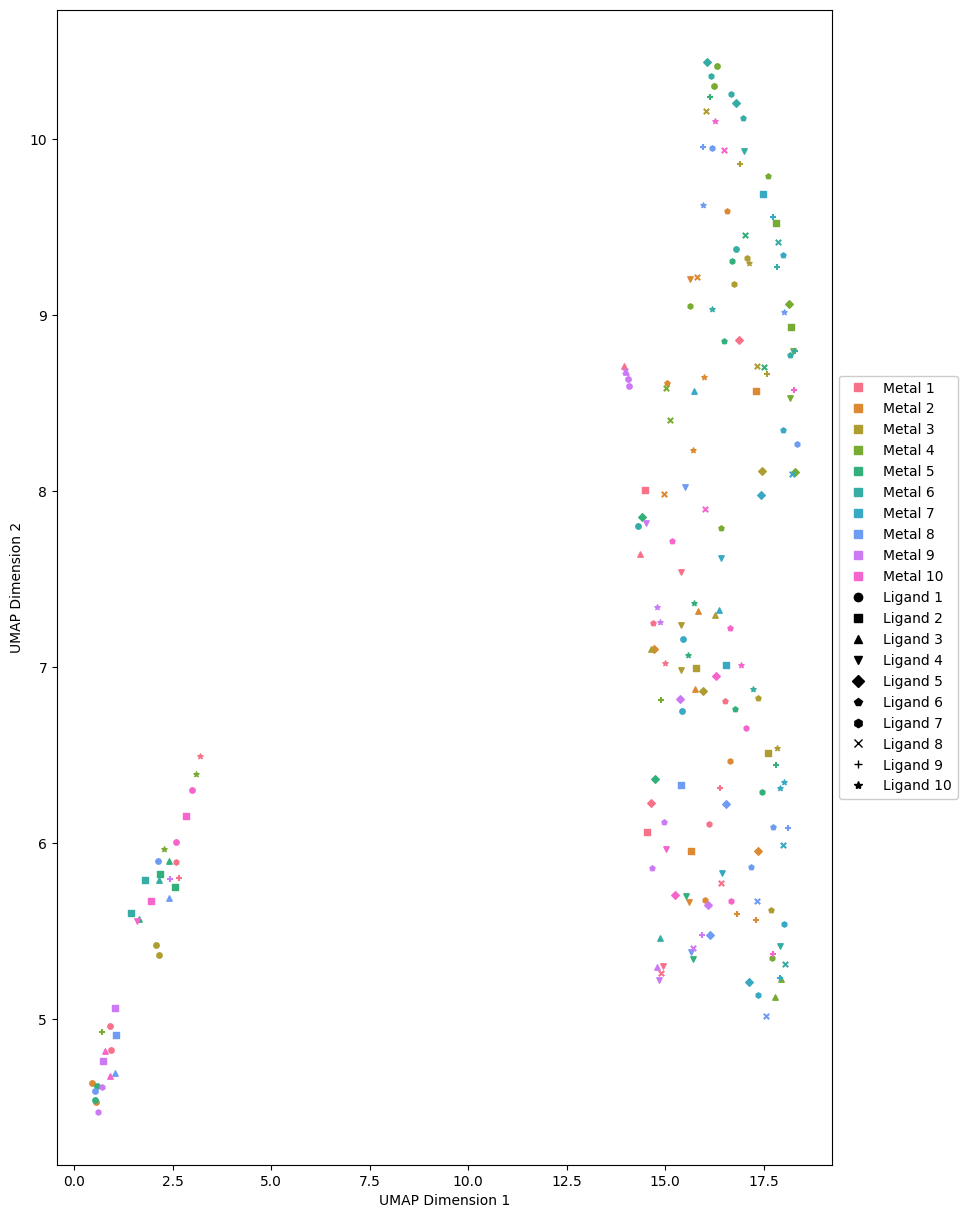
\includegraphics[width=1.0\textwidth]{figures/dpv_umap.png}
    \caption{Differential Pulse Voltammetry UMAP Projection}
    \label{dpv-umap}
\end{figure}
UMAP tends to focus more on preserving global structure and maintaining relative distance between clusters. Therefore, clusters in the UMAP plot are usually well-separated and evenly distributed. UMAP tries to preserve local and global neighborhoods, resulting in more evenly spaced clusters and better representation of both local and global structures. UMAP embeddings are generally more stable across different runs and parameter settings compared to t-SNE. Figures \ref{cv-umap} and \ref{dpv-umap} illustrate these characteristics, especially when contrasted with the projections generated by t-SNE.

Utilizing machine learning techniques to classify voltammetry data based on the overall shape presents numerous benefits over merely employing a script to identify the number of peaks, as has traditionally been done. Machine learning models can be trained to recognize patterns and variations regarding the overall shape and number of peaks. They can adapt to experimental conditions, electrode materials, and analytes without needing manual adjustment of parameters. Voltammetry data can often be noisy, especially at low concentrations. ML models can be trained to distinguish true peaks from noise more effectively than simple peak-finding algorithms. Voltammograms can vary in characteristics due to factors such as electrode deterioration, surface roughness, and solution composition. ML models can learn to handle this variability and provide more reliable peak classification across different experimental conditions. Additionally, ML models can learn when the electrode deteriorates and automatically polish it. ML models can automatically extract relevant features from voltammogram data such as peak heights, peak widths, peak potential, and overall shape. This allows for more comprehensive analysis beyond locating peaks. Once trained, ML models can be integrated into larger data analysis pipelines to classify cyclic voltammetry data rapidly and efficiently, potentially saving time and effort compared to manual analysis or parameter tuning for peak-finding algorithms. These automated analysis techniques can be integrated into an SDL, updating them with newly generated data to increase their accuracy as more experiments are performed.

In summary, clustering techniques play a crucial role in analyzing and interpreting experimental voltammetry results obtained from SDLs. By organizing data into meaningful clusters, clustering techniques like K-Means and DBSCAN and dimensionality reduction techniques like t-SNE and UMAP uncover patterns, similarities, and trends that enhance our understanding of the electrochemical compounds of interest. The choice of appropriate clustering algorithms and parameter selection methods, such as the Elbow Method and Silhouette Method, have been discussed to ensure meaningful and reliable clustering results. The results obtained from clustering algorithms and dimensionality reduction techniques have provided valuable insights into the underlying structure of the experimental data, facilitating compound identification, error detection, and decision-making processes in SDLs.
\chapter{Classification} \label{chap:chap-3}


% add citation for the chapter if it is a reprint


% remove the following and add your chapter text
\section{Introduction}
A classifier was trained to predict what metals and ligands were used to generate each voltammogram to demonstrate further the feasibility of using this encoding technique for various machine learning tasks. It is important to note that the dataset used is relatively small for a deep learning task. For training, the dataset was split with 80\% for training, 10\% for validation, and 10\% for testing. 5-fold cross-validation, a technique for assessing the performance of a machine learning model by dividing the dataset into k subsets, training the model on k-1 subsets, and evaluating it on the remaining subset for each subset, is also used \cite{hastie_09_elements-of.statistical-learning}. An important insight to consider is the similarity between voltammetry data and images. After all, each point has a potential and current value, similar to an image\textquotesingle s RGB values. The main difference is that an image is 2-dimensional while voltammetry data is 1-dimensional. Many previous works have used convolutional neural networks (CNNs) for classification tasks \cite{SHARMA2018377}. Using this as inspiration, the proposed model architecture for voltammetry data classification uses 1-dimensional convolutional layers. 
\section{Variational Autoencoders}
\begin{figure}[h!]
  \centering
    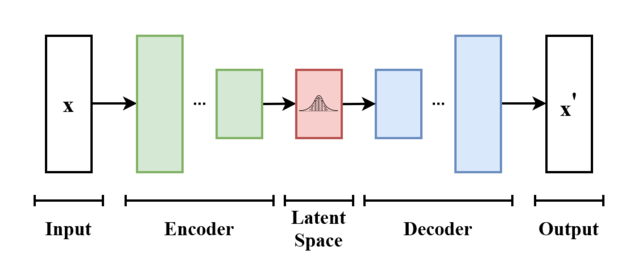
\includegraphics[width=1.0\textwidth]{figures/autoencoder_architecture.png}
    \caption{Autoencoder Diagram}
    \label{autoencoder_diagram}
    Input is encoded into latent space and then recreated using decoder
\end{figure}
Since one major challenge is the dataset size, one method to address this is to create synthetic data. 
A variational autoencoder (VAE) is similar to the autoencoder neural network architecture shown in Figure \ref{autoencoder_diagram}, with the main difference being that VAEs connects the encoder to its decoder through a probabilistic latent space that corresponds to the parameters of a variational distribution \cite{PinheiroCinelli2021}. The encoder maps each point from the dataset into a distribution within the latent space rather than a single point in that space. The distribution is typically Gaussian with a mean and a variance. Once the VAE is trained, different points can be sampled from the learned latent space distribution. These samples represent different configurations of the input data in the latent space. The sampled points from the latent space are fed into the decoder network, which reconstructs the input data corresponding to those points and generates a diverse set of synthetic data samples that resemble the original data distribution. The variability in the latent space allows for the generation of novel and diverse data samples that capture the underlying characteristics of the training data.
\section{Conditional Variational Autoencoders}
While traditional VAEs learn a latent space for the dataset, conditional variational autoencoders (CVAEs) expand this concept by introducing conditional dependencies between the input data and the latent variables. In the context of generating synthetic data, CVAEs offer a more controlled approach by allowing the generation process to be conditioned on additional information, such as class labels or other attributes associated with the data.
By conditioning the generation process on known attributes or labels, CVAEs can generate synthetic data samples that capture the underlying data distribution and adhere to specific conditions or constraints defined by the conditioning variables. This enables the targeted generation of synthetic data for different classes or categories when labelled data is lacking. In this case, the metal and ligand are encoded using one-hot encoding and passed to the decoder to generate data from the same class. 
\section{Classifier Model Architecture}
\begin{figure}[!h]
  \centering
    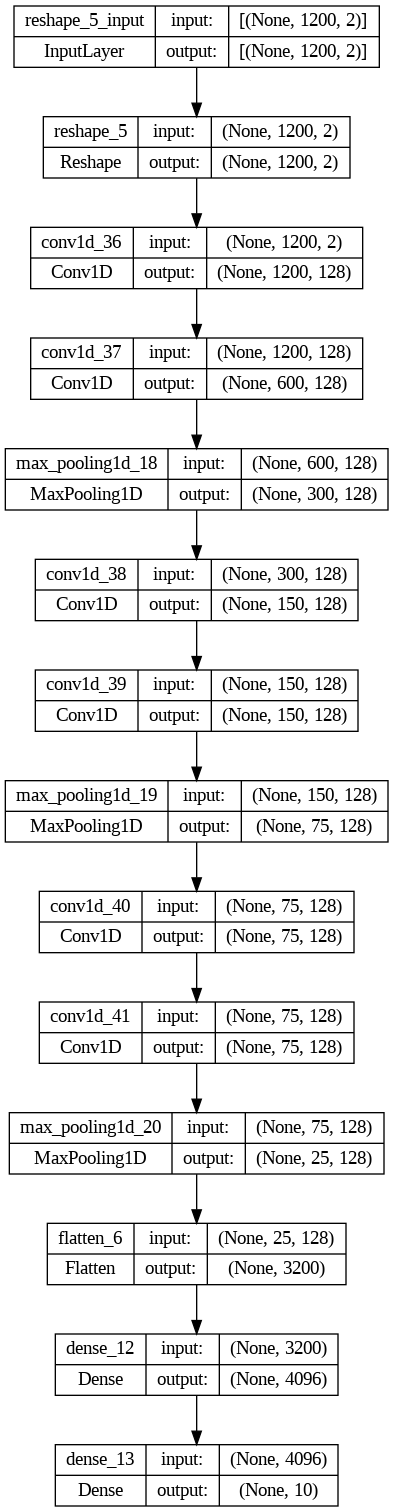
\includegraphics[width=0.25\textwidth]{figures/model_architecture.png}
    \caption{Classification Model Architecture}
    \label{model_arch}
\end{figure}
The classifier architecture can be seen in Figure \ref{model_arch}. The model consists of several convolutional and max-pooling layers to encode the data and reduce dimensions. All layers except for the output layer use the ReLU activation function. The output layer is a dense layer with ten units, one for each metal/ligand, and a softmax activation function. The Adam optimizer and categorical cross-entropy loss are used to train the model. Additionally, the model uses L2 regularization and early stopping to prevent overfitting and ensure smooth convergence. The Glorot uniform initializer is used for weight initialization to facilitate better gradient flow and prevent exploding gradients. 
\section{Results and Discussion}
\begin{table}[!h]
\begin{center}
\begin{tabular}{c|c|c|c|c|c|c}
Model & Fold 1 Acc & Fold 2 Acc & Fold 3 Acc & Fold 4 Acc & Fold 5 Acc & Avg Acc\\
\hline
CV Ligands & 75.13\% & 80.29\% & 69.65\% & 76.40\% & 78.82\% & 76.06\%\\
CV Metals & 79.24\% & 82.50\% & 81.36\% & 80.11\% & 78.97\% & 80.44\%\\
DPV Ligands & 30.00\% & 35.00\% & 25.00\% & 25.00\% & 30.00\% & 29.00\%\\
DPV Metals & 25.00\ & 30.00\% & 25.00\% & 20.00\% & 25.00\% & 25.00\%\\
\end{tabular}
\caption{Classification Accuracy}
\label{classification_results}
\end{center}
\end{table}
Separate classifiers were trained, each with a unique task of classifying CV ligands, CV metals, DPV ligands, and DPV metals. 
The accuracy of the classifiers can be seen in Table \ref{classification_results}, and the results were much better for the CV data than the DPV data. This difference can likely be attributed to the size of the datasets. 
\begin{table}[!h]
\begin{center}
\begin{tabular}{c|c|c|c|c|c|c}
Model & Fold 1 Acc & Fold 2 Acc & Fold 3 Acc & Fold 4 Acc & Fold 5 Acc & Avg Acc \\
\hline
CV Ligands & 77.86\% & 78.50\% & 80.94\% & 72.01\% & 73.02\% & 76.47\%\\
CV Metals & 85.00\% & 81.23\% & 84.19\% & 83.10\% & 78.75\% & 82.45\%\\
DPV Ligands & 25.00\% & 25.00\% & 15.00\% & 20.00\% & 20.00\% & 21.00\%\\
DPV Metals & 25.00\% & 20.00\% & 20.00\% & 25.00\% & 25.00\% & 23.00\%
\end{tabular}
\caption{Classification Accuracy with Synthetic Data}
\label{vae_classification_results}
\end{center}
\end{table}
After incorporating synthetic data generated with the CVAE into the training process, accuracy significantly improved for classifying CV data, as seen in Table \ref{vae_classification_results}. However, the DPV ligands classifier saw a decrease in performance. Again, this is likely due to the size of the dataset. Several key considerations impact the quality of data generated by VAEs, especially when dealing with small datasets. Firstly, the quality and diversity of the original data influence the effectiveness of the synthetic data produced by VAEs. With limited variation or complexity in a small dataset, the VAE might struggle to accurately capture the proper underlying data distribution, potentially resulting in synthetic data that fails to represent the characteristics of the actual data fully. This mismatch can detrimentally affect classifier performance. 

Additionally, the risk of overfitting is heightened in small datasets, where the classifier may excessively specialize in training data patterns that do not generalize well. Introducing synthetic data from a VAE can compound this issue if the VAE itself overfits the small dataset, producing synthetic data overly similar to the training data, which provides minimal additional information for the classifier and can lead to decreased performance on unseen data. VAEs implicitly learn the probability distribution of the input data. However, suppose the actual data distribution is significantly different from the distribution learned by the VAE due to the small dataset size. In that case, the synthetic data generated by the VAE may not accurately represent the true data distribution. This distribution mismatch can confuse the classifier, as it may encounter data points in the synthetic dataset that deviate from the real data distribution, leading to suboptimal performance.
\begin{table}[!h]
\begin{center}
\begin{tabular}{c|c|c|c|c}
 & Precision & Recall & F1-Score & Support\\
\hline
Metal 1 & 0.88 & 0.88 & 0.88 & 8\\
Metal 2 & 0.80 & 1.00 & 0.89 & 8\\
Metal 3 & 1.00 & 1.00 & 1.00 & 4\\
Metal 4 & 1.00 & 0.83 & 0.91 & 12\\
Metal 5 & 1.00 & 0.71 & 0.83 & 7\\
Metal 6 & 0.88 & 0.78 & 0.82 & 9\\
Metal 7 & 0.82 & 0.90 & 0.86 & 10\\
Metal 8 & 0.50 & 0.40 & 0.44 & 5\\
Metal 9 & 0.78 & 1.00 & 0.88 & 7\\
Metal 10 & 0.82 & 0.90 & 0.86 & 10\\
\hline
Accuracy & & & 0.85 & 80\\
Macro Avg & 0.85 & 0.84 & 0.84 & 80\\
Weighted Avg & 0.86 & 0.85 & 0.85 & 80
\end{tabular}
\caption{CV Metals Classification Report}
\label{cv_metal_report}
\end{center}
\end{table}
Table \ref{cv_metal_report} provides insights into the precision, recall, and F1-score when classifying each metal type, along with the number of instances (support) for each metal type. Precision indicates the proportion of true positive predictions among all positive predictions, while recall measures the proportion of true positives that were correctly identified. F1-score, the harmonic mean of precision and recall, provides a balanced measure between the two.
Overall, the classifier model achieved an accuracy of 85\%, indicating its effectiveness in classifying different metal types. However, it is important to note variations in performance across metal types. For instance, Metal 3 achieved perfect precision, recall, and F1-score, suggesting the model\textquotesingle s ability to  classify this particular metal type accurately. On the other hand, Metal 8 exhibited lower precision and recall scores, indicating potential challenges in distinguishing this metal type from others.
Both macro-average and weighted-average metrics hover around 0.85, indicating a reasonably balanced performance across all metal types. These metrics consider the average performance across all classes, with macro-average treating all classes equally, while weighted-average considers the contribution of each class based on its support.
\begin{table}[!h]
\begin{center}
\begin{tabular}{c|c|c|c|c}
 & Precision & Recall & F1-Score & Support\\
\hline
Ligand 1 & 0.88 & 0.78 & 0.82 & 9\\
Ligand 2 & 0.88 & 0.88 & 0.88 & 8\\
Ligand 3 & 0.75 & 0.86 & 0.80 & 7\\
Ligand 4 & 0.45 & 0.71 & 0.56 & 7\\
Ligand 5 & 0.78 & 0.70 & 0.74 & 10\\
Ligand 6 & 1.00 & 0.86 & 0.92 & 7\\
Ligand 7 & 0.71 & 0.50 & 0.59 & 10\\
Ligand 8 & 0.67 & 0.89 & 0.76 & 9\\
Ligand 9 & 1.00 & 0.67 & 0.80 & 3\\
Ligand 10 & 1.00 & 0.90 & 0.95 & 10\\
\hline
Accuracy & & & 0.78 & 80\\
MacroAvg & 0.81 & 0.77 & 0.78 & 80\\
WeightedAvg & 0.80 & 0.78 & 0.78 & 80
\end{tabular}
\caption{CV Ligands Classification Report}
\label{cv_ligands_report}
\end{center}
\end{table}
Table \ref{cv_metal_report} shows the classification report for classifying ligands. The classifier achieved an accuracy of 78\% overall, indicating its capability to classify different metal types to some extent. However, upon closer examination, there are notable variations in performance across metal types. For instance, Metal 6 demonstrates excellent precision, recall, and F1-score, suggesting the model\textquotesingle s proficiency in accurately classifying this metal type. Conversely, Metal 4 exhibits lower precision, recall, and F1-score, indicating challenges in distinguishing this metal type from others.
\begin{table}[!h]
\begin{center}
\begin{tabular}{c|c|c|c|c}
 & Precision & Recall & F1-Score & Support\\
\hline
Ligand 1 & 1.00 & 1.00 & 1.00 & 1\\
Ligand 2 & 0.00 & 0.00 & 0.00 & 2\\
Ligand 3 & 0.33 & 0.25 & 0.29 & 4\\
Ligand 4 & 0.33 & 0.33 & 0.33 & 3\\
Ligand 5 & 0.50 & 0.50 & 0.50 & 4\\
Ligand 6 & 0.00 & 0.00 & 0.00 & 1\\
Ligand 7 & 0.00 & 0.00 & 0.00 & 1\\
Ligand 8 & 0.00 & 0.00 & 0.00 & 0\\
Ligand 9 & 0.00 & 0.00 & 0.00 & 1\\
Ligand 10 & 1.00 & 0.33 & 0.50 & 3\\
\hline
Accuracy & & & 0.30 & 20\\
MacroAvg & 0.32 & 0.24 & 0.26 & 20\\
WeightedAvg & 0.42 & 0.30 & 0.33 & 20
\end{tabular}
\caption{DPV Ligands Classification Report}
\label{dpv_ligand_report}
\end{center}
\end{table}
\begin{table}[!h]
\begin{center}
\begin{tabular}{c|c|c|c|c}
 & Precision & Recall & F1-Score & Support\\
\hline
Ligand 1 & 0.33 & 1.00 & 0.50 & 2\\
Ligand 2 & 0.00 & 0.00 & 0.00 & 1\\
Ligand 3 & 0.25 & 0.50 & 0.33 & 2\\
Ligand 4 & 0.00 & 0.00 & 0.00 & 3\\
Ligand 5 & 0.00 & 0.00 & 0.00 & 1\\
Ligand 6 & 0.50 & 0.25 & 0.33 & 4\\
Ligand 7 & 0.00 & 0.00 & 0.00 & 2\\
Ligand 8 & 1.00 & 0.50 & 0.67 & 2\\
Ligand 9 & 0.00 & 0.00 & 0.00 & 3\\
Ligand 10 & 0.00 & 0.00 & 0.00 & 0\\
\hline
Accuracy & & & 0.30 & 20\\
MacroAvg & 0.23 & 0.25 & 0.20 & 20\\
WeightedAvg & 0.26 & 0.25 & 0.22 & 20
\end{tabular}
\caption{DPV Metals Classification Report}
\label{dpv_metal_report}
\end{center}
\end{table}
Table \ref{dpv_ligand_report} and Table \ref{dpv_metal_report} show the classification reports for DPV ligands and metals. However, the small sample size makes it difficult to draw definitive conclusions from this data. To further assess the performance of these classification models, receiving operating characteristic (ROC) curves and area under the ROC curve (AUC) values can be used to gain valuable insights into the discrimination capabilities and robustness of the models when distinguishing between various metals and ligands. ROC curves and AUC values help assess the robustness of the classification model by showing how well it performs across different thresholds and levels of noise. A smooth ROC curve with a high AUC suggests that the model can reliably discriminate between different metals and ligands even in the presence of noise or variability. 

Furthermore, there may be a need to choose a classification threshold that balances sensitivity and specificity according to specific requirements or constraints. ROC curves provide a visual aid for selecting an appropriate threshold based on the desired trade-off between true positives and false positives. For example, when integrating with an SDL, minimizing false positives (misclassification of metals or ligands) might be prioritized over maximizing true positives.
\begin{figure}[h!]
  \centering
    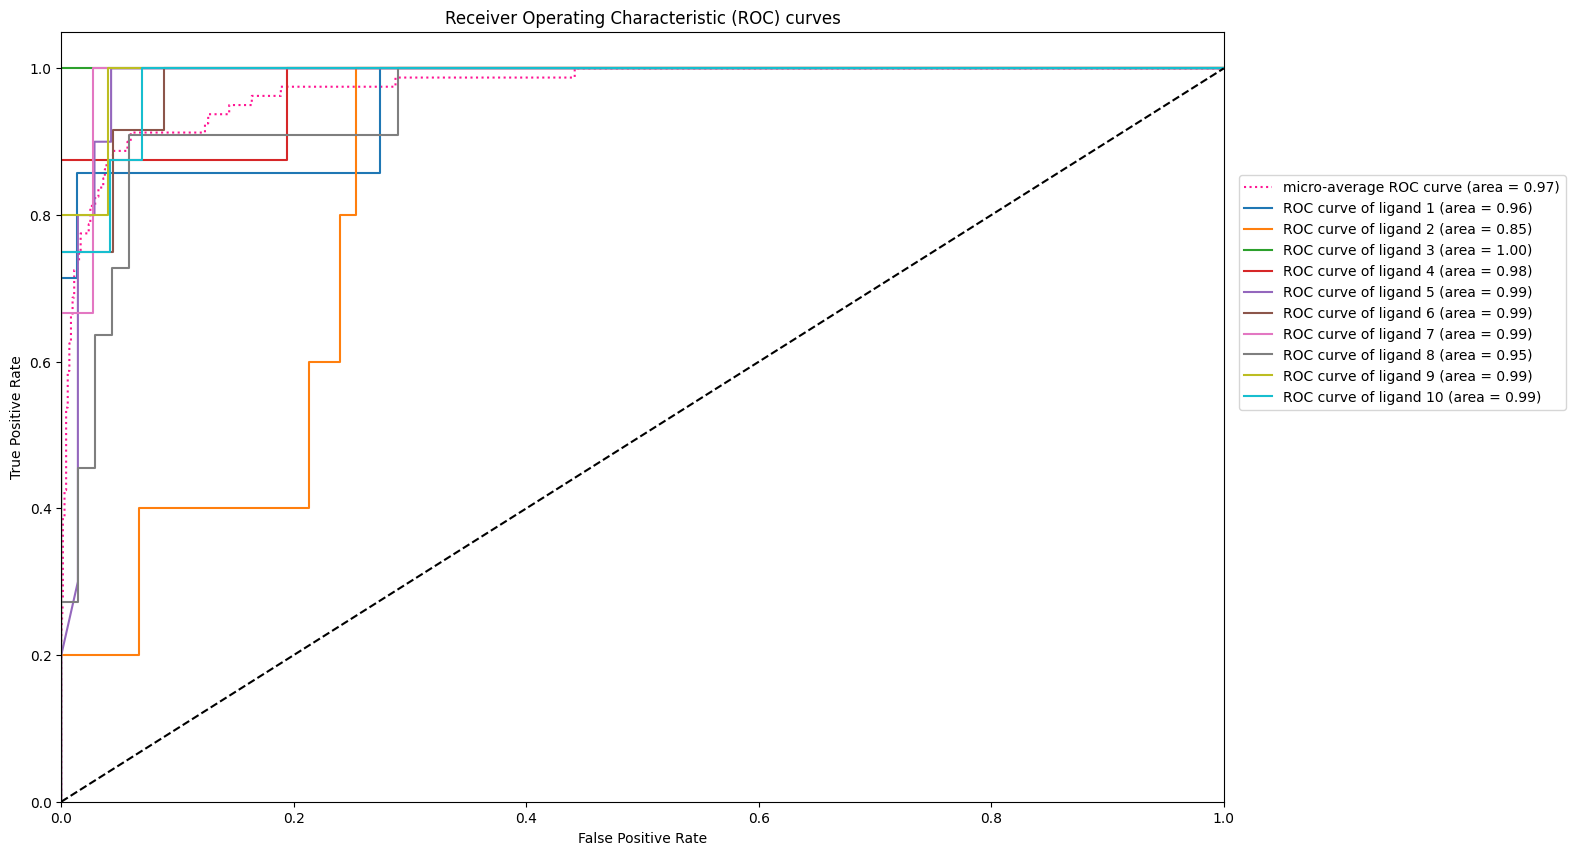
\includegraphics[width=1.0\textwidth]{figures/ligand_roc.png}
    \caption{CV Ligand ROC Curves}
    \label{ligand_roc}
\end{figure}
\begin{figure}[h!]
  \centering
    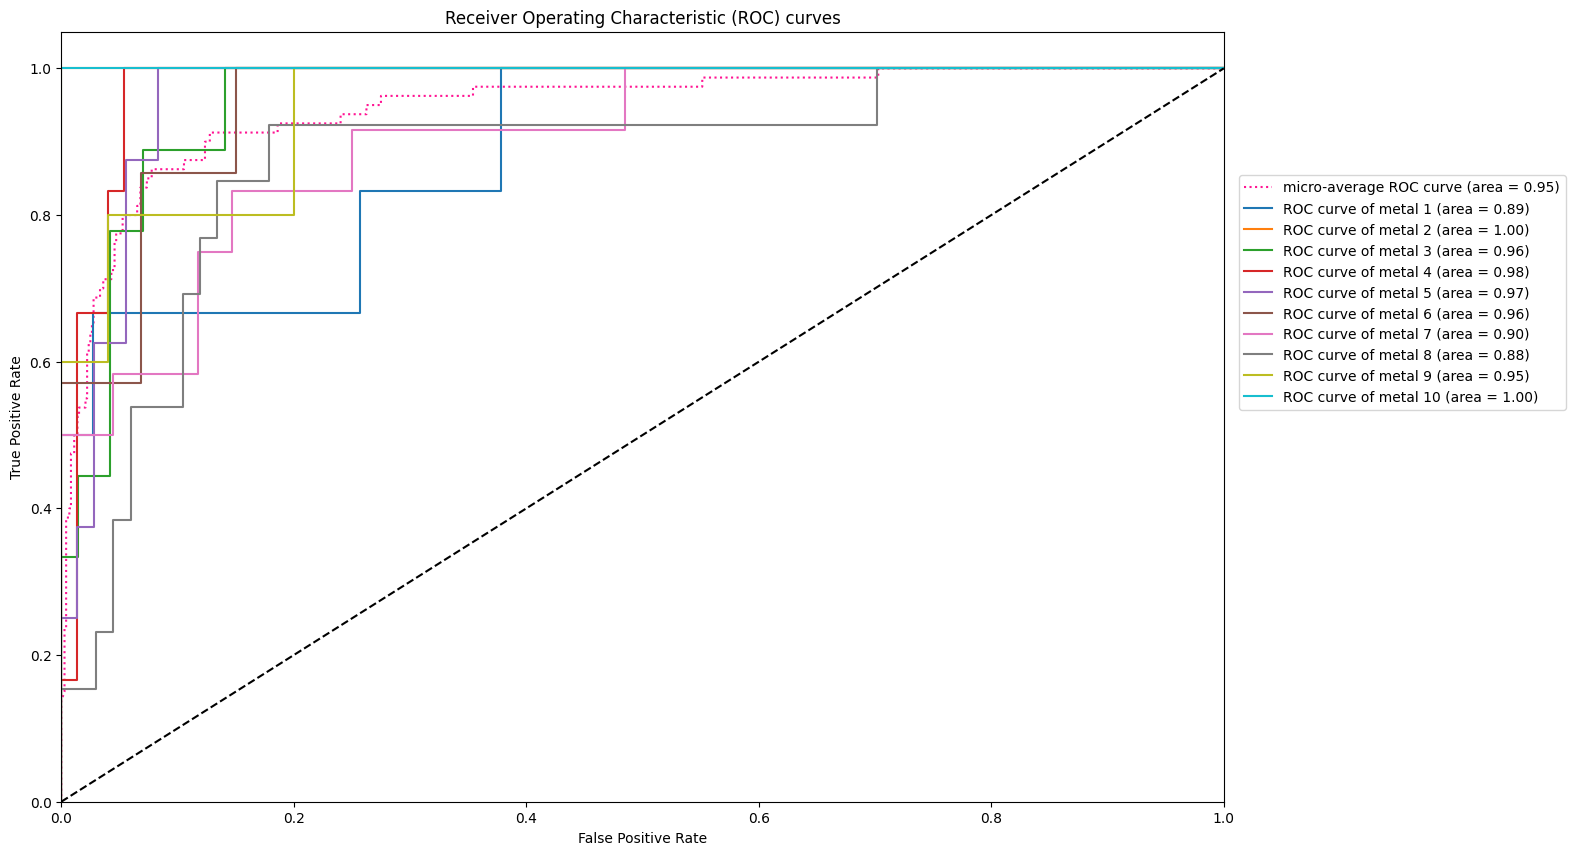
\includegraphics[width=1.0\textwidth]{figures/metal_roc.png}
    \caption{CV Metal ROC Curves}
    \label{metal_roc}
\end{figure}
The ROC curves in Figure \ref{ligand_roc} and Figure \ref{metal_roc} show good results for both metals and ligands. The area under the ROC curve (AUC) calculation summarized the ROC curve analysis into a scalar value, which ranges between 0 and 1. The closer the AUC score to value 1, the better the application’s overall performance.
\begin{figure}[h!]
  \centering
    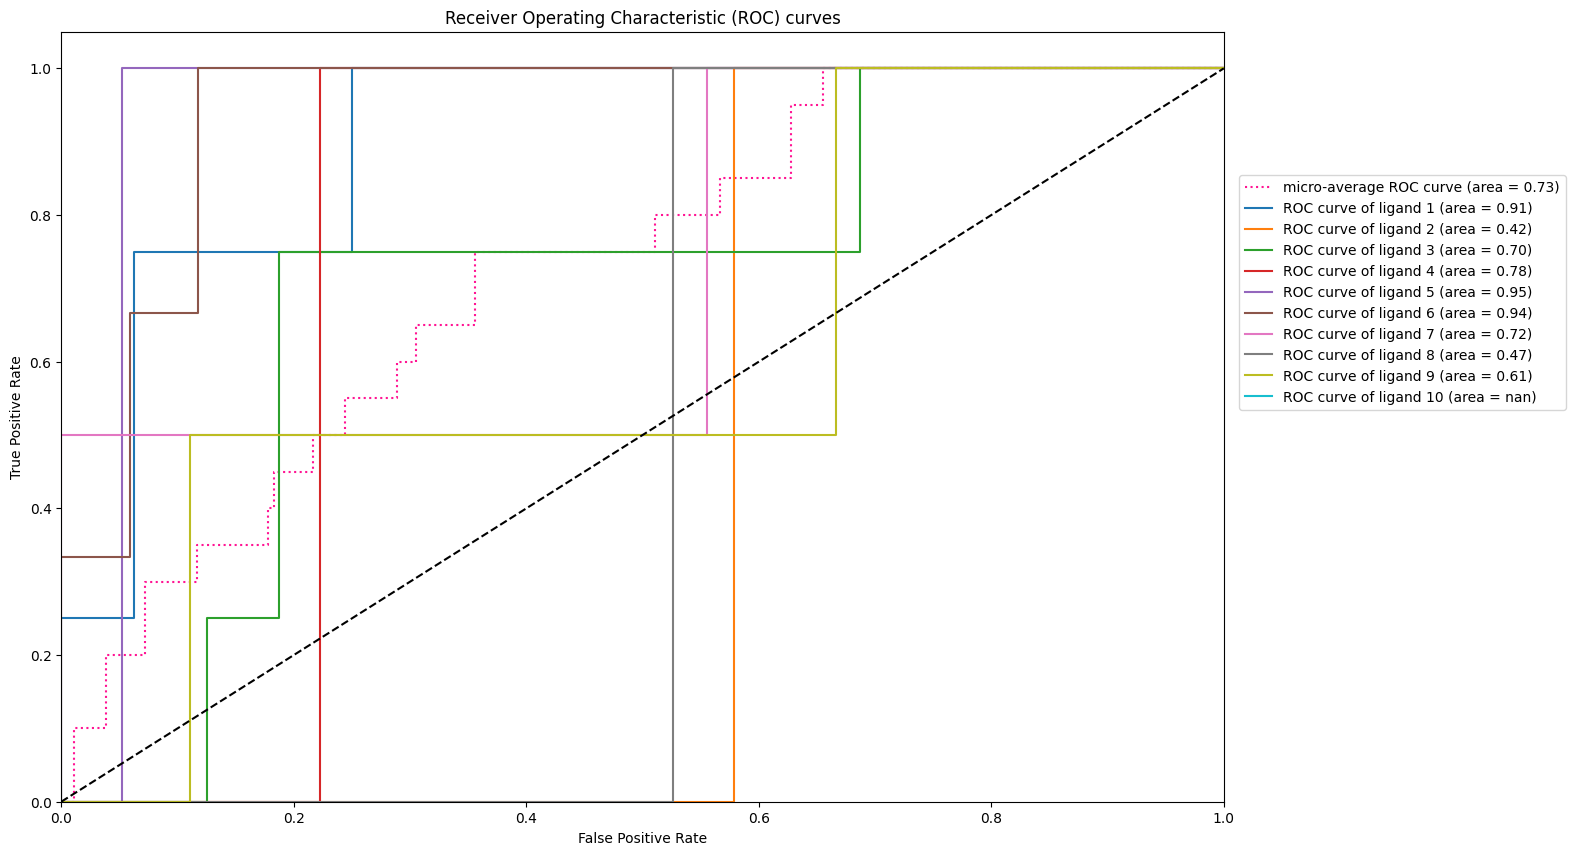
\includegraphics[width=1.0\textwidth]{figures/dpv_ligand_roc.png}
    \caption{DPV Ligand ROC Curves}
    \label{dpv_ligand_roc}
\end{figure}
\begin{figure}[h!]
  \centering
    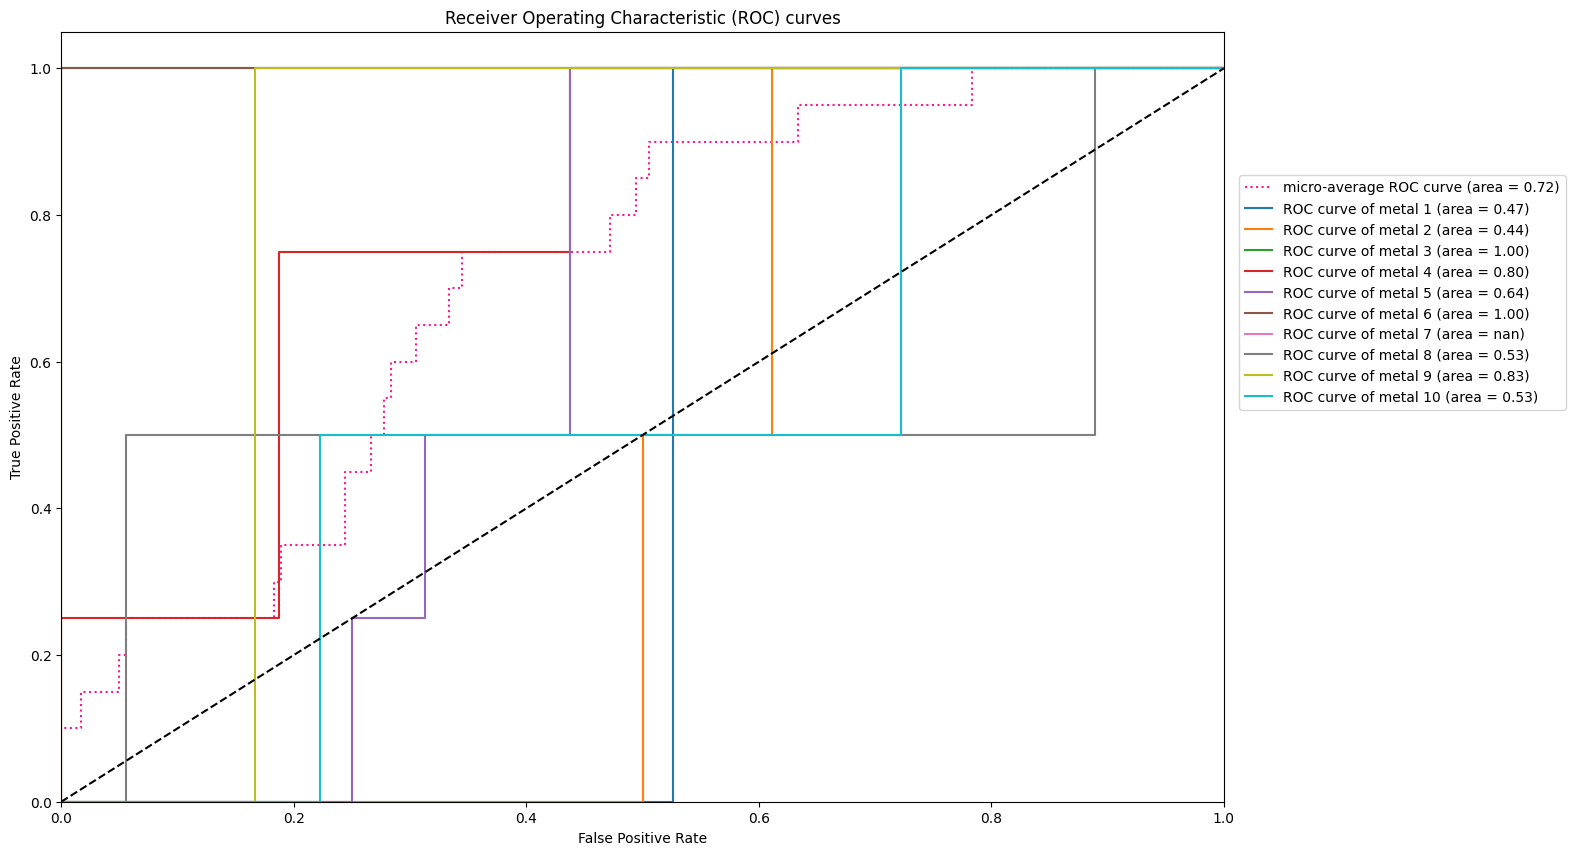
\includegraphics[width=1.0\textwidth]{figures/dpv_metal_roc.png}
    \caption{DPV Metal ROC Curves}
    \label{dpv_metal_roc}
\end{figure}
In Figure \ref{dpv_ligand_roc} and Figure \ref{dpv_metal_roc}, the ROC curves show that the classifier outperforms a random classifier by having an AUC value above 0.5. 
\begin{figure}[h!]
  \centering
    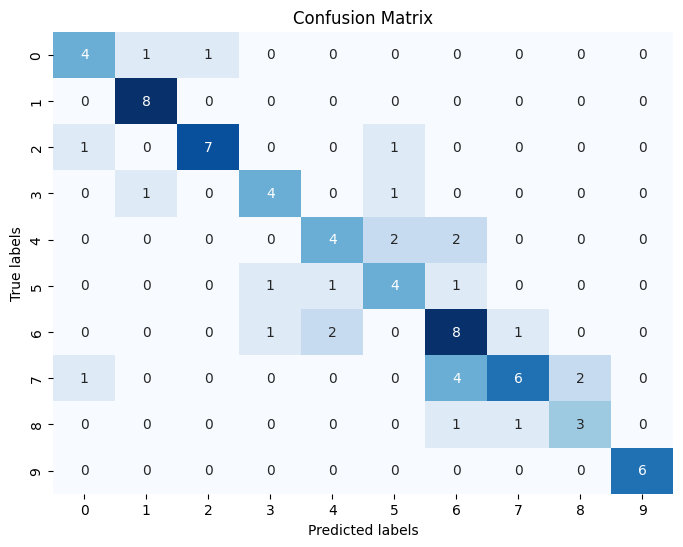
\includegraphics[width=1.0\textwidth]{figures/cv_ligand_matrix.png}
    \caption{CV Ligand Confusion Matrix}
    \label{cv_ligand_matrix}
\end{figure}
The data itself may cause issues with classification as some ligands and metals may be more difficult to distinguish than others. The confusion matrices are provided to investigate this.
From the confusion matrix for ligands \ref{cv_ligand_matrix}, ligand seven was often misclassified as ligand six.
\begin{figure}[h!]
  \centering
    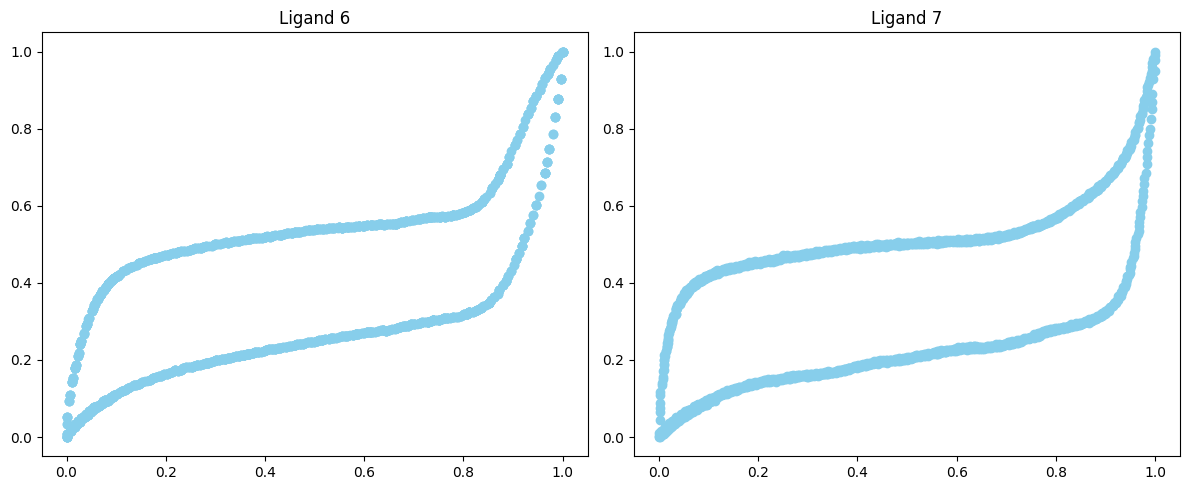
\includegraphics[width=1.0\textwidth]{figures/ligand_comparison.png}
    \caption{Ligand Six and Ligand Seven Voltammogram Comparison}
    \label{ligand_comparison}
\end{figure}
However, this misclassification is understandable. Figure \ref{ligand_comparison} shows that the voltammograms for ligand six and ligand seven are quite similar. 
\begin{figure}[h!]
  \centering
    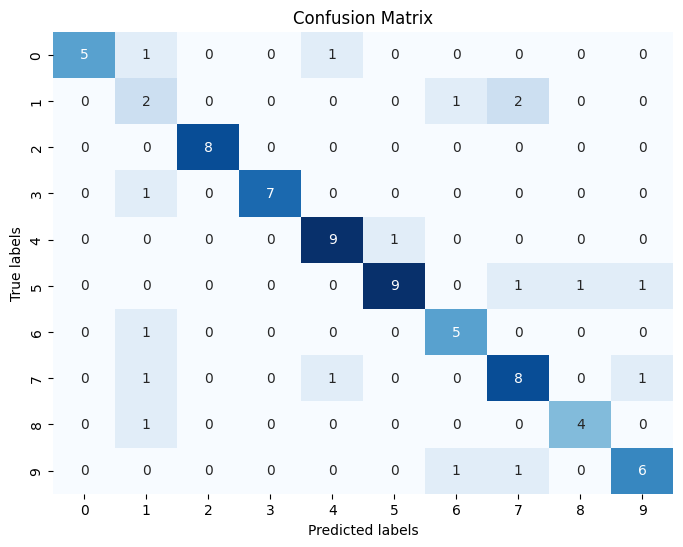
\includegraphics[width=1.0\textwidth]{figures/cv_metal_matrix.png}
    \caption{CV Metal Confusion Matrix}
    \label{cv_metal_matrix}
\end{figure}
From the confusion matrix for metals \ref{cv_metal_matrix}, metal one was difficult to recognize, with many metals being misclassified as metal one. 
\begin{figure}[h!]
  \centering
    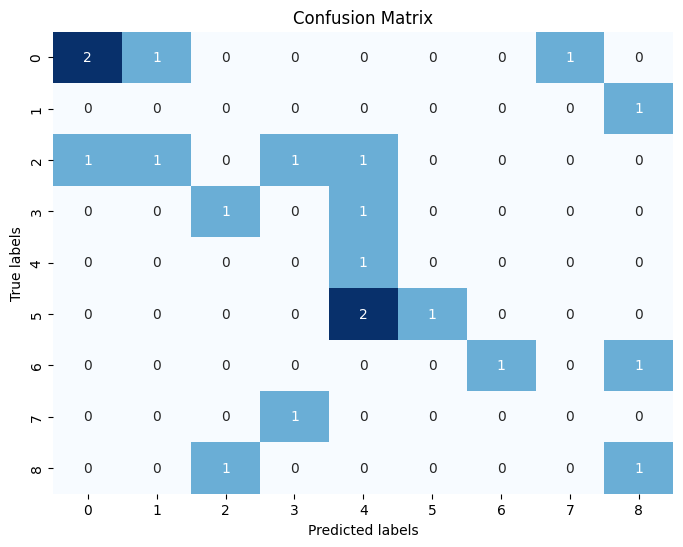
\includegraphics[width=1.0\textwidth]{figures/dpv_ligand_matrix.png}
    \caption{DPV Ligand Confusion Matrix}
    \label{dpv_ligand_matrix}
\end{figure}
\begin{figure}[h!]
  \centering
    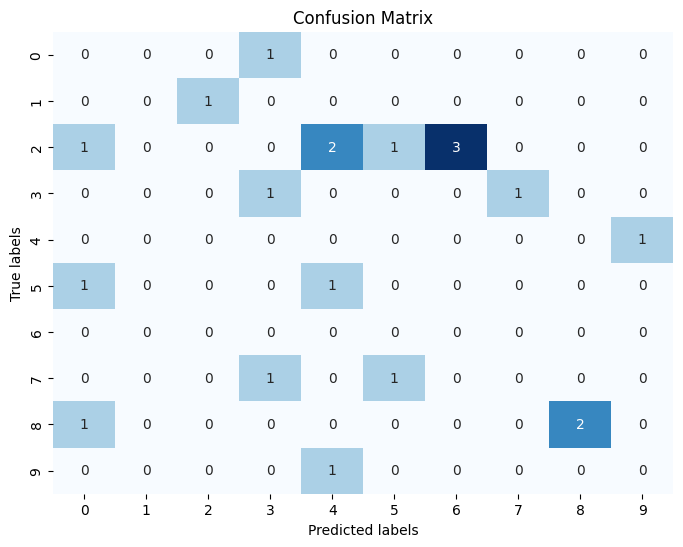
\includegraphics[width=1.0\textwidth]{figures/dpv_metal_matrix.png}
    \caption{DPV Metal Confusion Matrix}
    \label{dpv_metal_matrix}
\end{figure}
From the DPV confusion matrices seen in Figure \ref{dpv_metal_matrix} and Figure \ref{dpv_ligand_matrix}, it is hard to draw any definitive conclusions due to the dataset size. 
A major challenge in supervised learning is providing good examples during training. However, despite using a small dataset, these results are promising. This study establishes that crude CV data obtained from an economical potentiostat can be effectively encoded using CNNs. It was also shown that VAEs and CVAEs can generate high-quality, generalizable synthetic data. These findings align with recent research demonstrating that deep learning models can efficiently process CV data \cite{Hoar2022}. Future research incorporate group SELFIES within the decoder layer to predict or select from a pool of candidate redox groups identified through voltammetry. 

\chapter{Denoising} \label{chap:chap-4}

\section{Introduction}
As the previously discussed dataset was generated using a low-cost potentiostat that lacks the accuracy of commercial options \cite{PabloGarca2024}, we attempt to improve the quality of the data obtained by this potentiostat by applying ML to denoise the raw data with the commercial potentiostat data as a reference.
\section{Autoencoder}
As previously shown in Figure \ref{autoencoder_diagram}, an autoencoder is a neural network used to learn an efficient low-dimensional encoding of data. An autoencoder consists of an encoder and a decoder. The encoder transforms the input data into an encoded representation, and the decoder attempts to recreate the data from the encoded representation. Since the goal is to try and improve the data quality, the commercial potentiostat data is used for the decoder instead. This way, the low-cost potentiostat data is used to create an encoded representation, and an equivalent commercial potentiostat data is decoded. The main problem to solve is how to pair results from the two potentiostats. While the metal and ligand used for each experiment are recorded, numerous other variables can influence the data. Therefore, the challenge revolves around accurately aligning the outcomes generated by the low-cost potentiostat with their counterparts from the commercial one. This alignment is crucial for ensuring the reliability and validity of the encoded representations created by the autoencoder. Without precise pairing, the encoded representations may not accurately capture the underlying patterns in the data, leading to suboptimal performance of the autoencoder. To address this challenge, the clustering technique previously described can be employed. By leveraging the recorded information on metals and ligands, combined with other relevant variables, similar experimental results can be grouped. This clustering process helps in identifying pairs of results that share comparable characteristics, despite potential variations introduced by the different potentiostats.
\section{Results and Discussion}

\begin{figure}[h!]
  \centering
    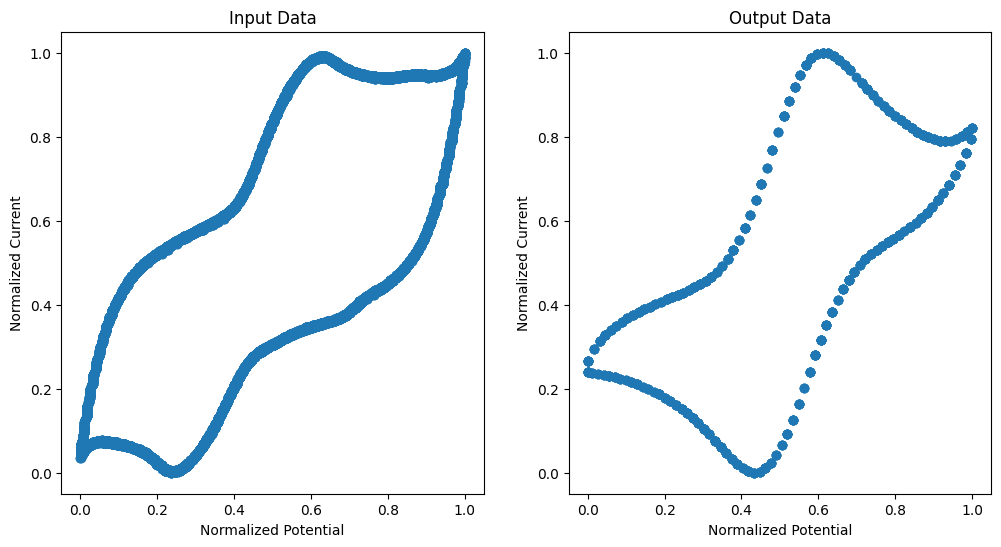
\includegraphics[width=1\textwidth]{figures/autoencoder.png}
    \caption{AutoEncoder Results}
    \label{autoncoder_results}
\end{figure}
In Figure \ref{autoncoder_results}, both the
As seen in Figure \ref{autoncoder_results}, both the input and output are similar in overall shape. However, the output contains a much more defined duck-shaped voltammogram, which is typically expected. The results show promising outcomes and indicate that an autoencoder can effectively transform data from the low-cost potentiostat to resemble data from the commercial potentiostat. By leveraging the capacity of deep neural networks to learn complex patterns and relationships within the data, it becomes feasible to enhance the quality of measurements obtained from low-cost instruments, thereby expanding their utility in research and industrial applications.
However, despite the promising results, several drawbacks and considerations must be acknowledged. Firstly, the effectiveness of the transformation heavily relies on the quality and diversity of the training data. Insufficient or biased training samples may lead to suboptimal performance and generalization issues, especially when dealing with complex electrochemical processes or diverse experimental conditions. While the autoencoder can effectively capture and replicate the dominant features present in the data, it may struggle with preserving subtle nuances or domain-specific characteristics inherent to the commercial potentiostat. Variations in hardware specifics, measurement protocols, or environmental factors could introduce discrepancies between the transformed and reference datasets. 
In conclusion, while autoencoders offer a promising avenue for enhancing the capabilities of low-cost potentiostats, their deployment must be accompanied by rigorous validation and consideration of the aforementioned limitations. Future research could focus on optimizing the autoencoder architecture, exploring alternative deep-learning techniques, and investigating strategies for addressing data heterogeneity to further improve the robustness and versatility of the proposed approach.

\chapter{Conclusion} \label{chap:chap-5}
In summary, the novel technique introduced for encoding CV and DPV data represents a pivotal advancement in the realm of SDLs. Shown through accurately segmenting voltammograms based on their characteristics and demonstrated efficacy across various machine learning tasks, including clustering, classification, denoising, and synthetic data generation, this technique signifies a significant step towards autonomous SDLs. Furthermore, its versatility extends beyond SDLs and can be applied to any 2-dimensional data. Moving forward, further exploration into alternative curve simplification algorithms and integration of the encoding technique into operational SDL frameworks stand as promising avenues for future research and development.

%% add more chapters as you need

%%%%%%%%%%%%%%%%%%%%%%%%%%%% END MAIN TEXT %%%%%%%%%%%%%%%%%%%%%%%%%%%%%





%%%%%%%%%%%%%%%%%%%%%%%%%%%%% BACK MATTER %%%%%%%%%%%%%%%%%%%%%%%%%%%%%%

%% references
\clearpage
\BibTextSpacing                     % single spacing for the bib items (too widespread otherwise)
% you can also change 'BibItemSeparation' variable to control the spacing
% header unnumbered chapters (to remove the headers, comment out the following line)
\fancyhead[L]{\nouppercase \leftmark}

\chap{Bibliographic references}


\nocite{*}
\printbibliography[heading=none]             % include reference chapter


%% appendix chapters
\MainTextSpacing                    % restoring double spacing for the contents in appendices
%% full header for appendix chapters (to remove the headers, comment out the following line)
\fancyhead[L]{\appendixname\ \thechapter. \nouppercase \leftmark}

%% necessary customization for the appendix and headers
\appendix 
\makeatletter
\addtocontents{toc}{\protect\renewcommand\protect\cftchappresnum{\@chapapp\ }}
\makeatother
\renewcommand{\thechapter}{\Alph{chapter}}
\label{appendix}

\chapter{CV K-Means Cluster Results}
Cluster 1:\\
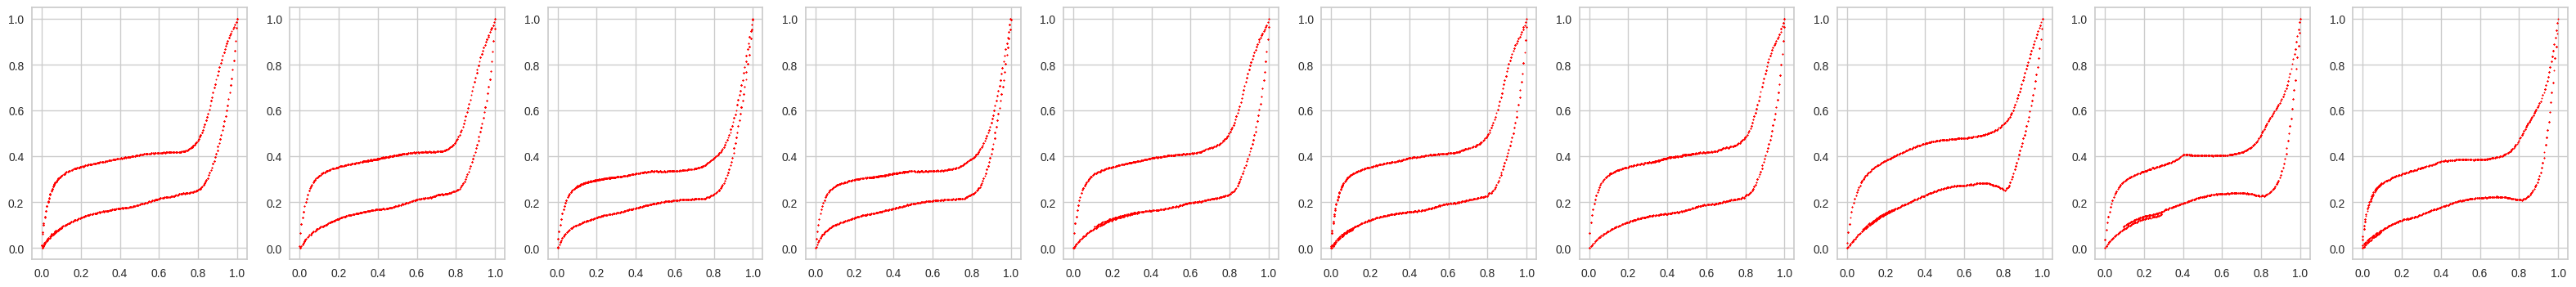
\includegraphics[width=1.0\textwidth]{figures/clusters/cv_cluster1.png}
Cluster 2:\\
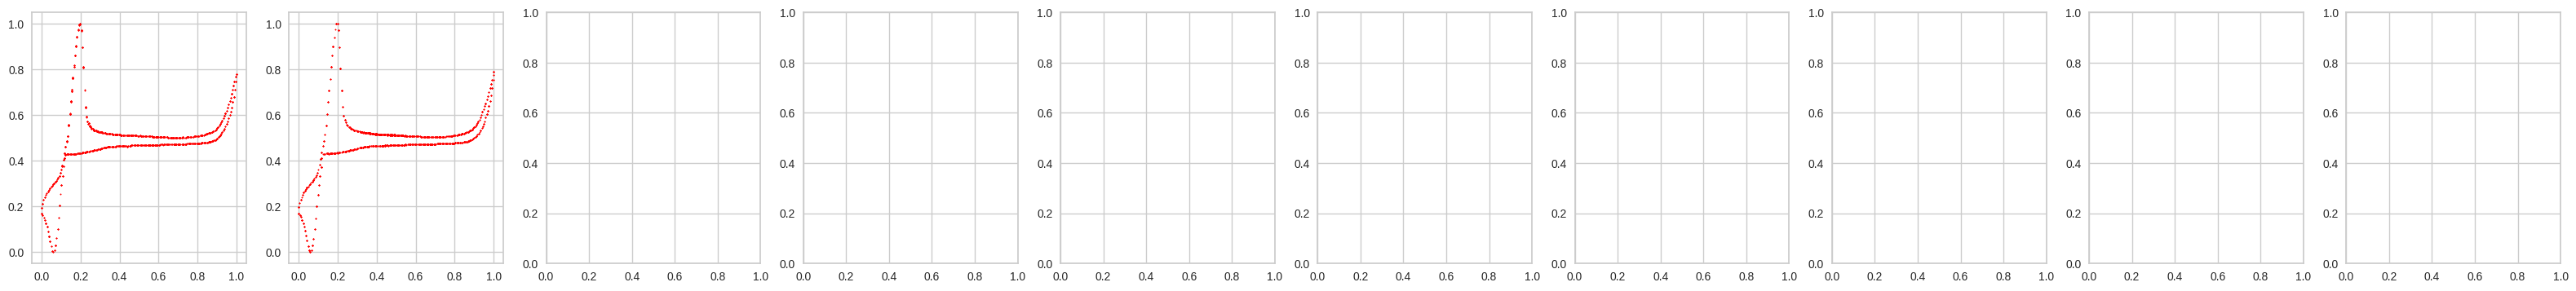
\includegraphics[width=1.0\textwidth]{figures/clusters/cv_cluster2.png}
Cluster 3:\\
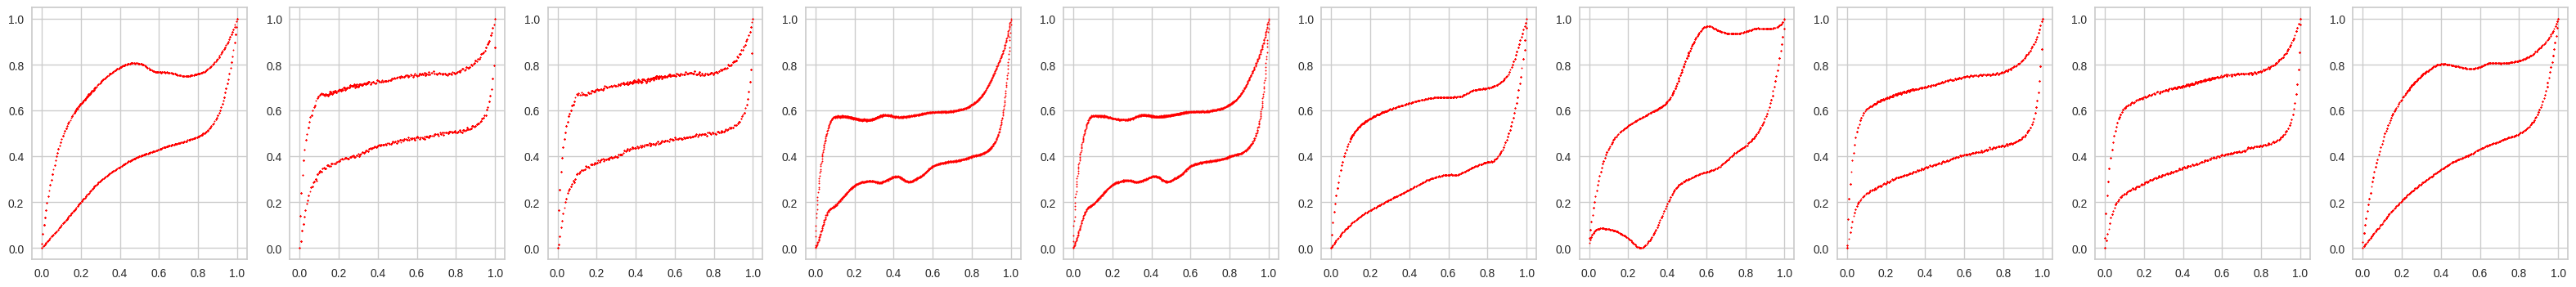
\includegraphics[width=1.0\textwidth]{figures/clusters/cv_cluster3.png}
Cluster 4:\\
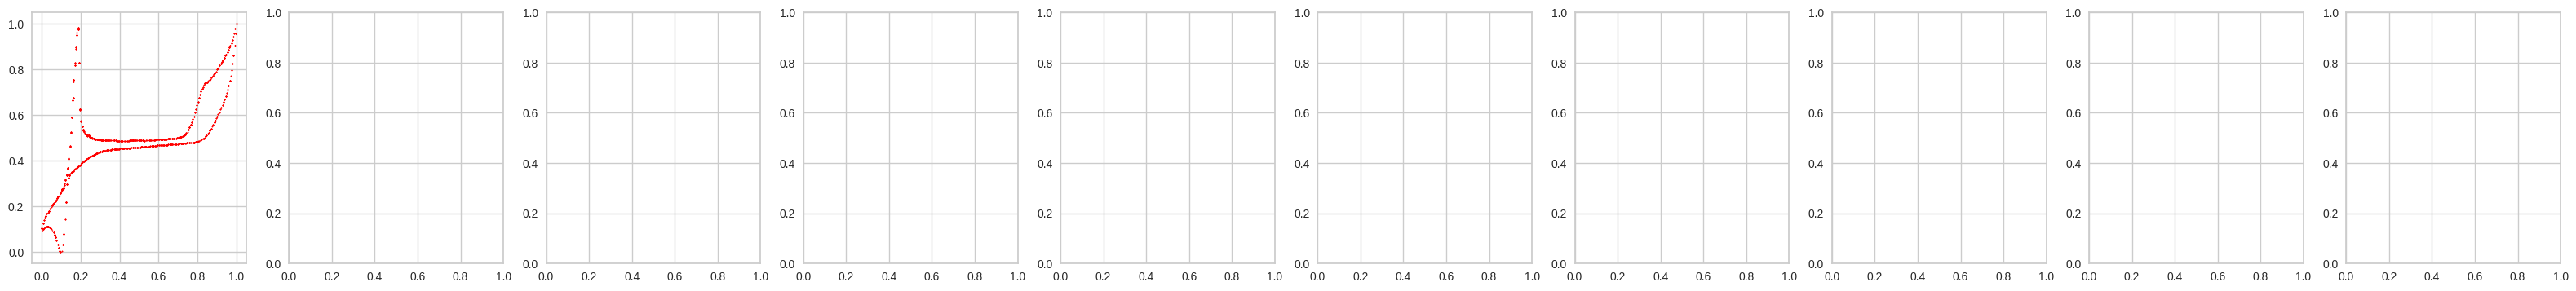
\includegraphics[width=1.0\textwidth]{figures/clusters/cv_cluster4.png}
Cluster 5:\\
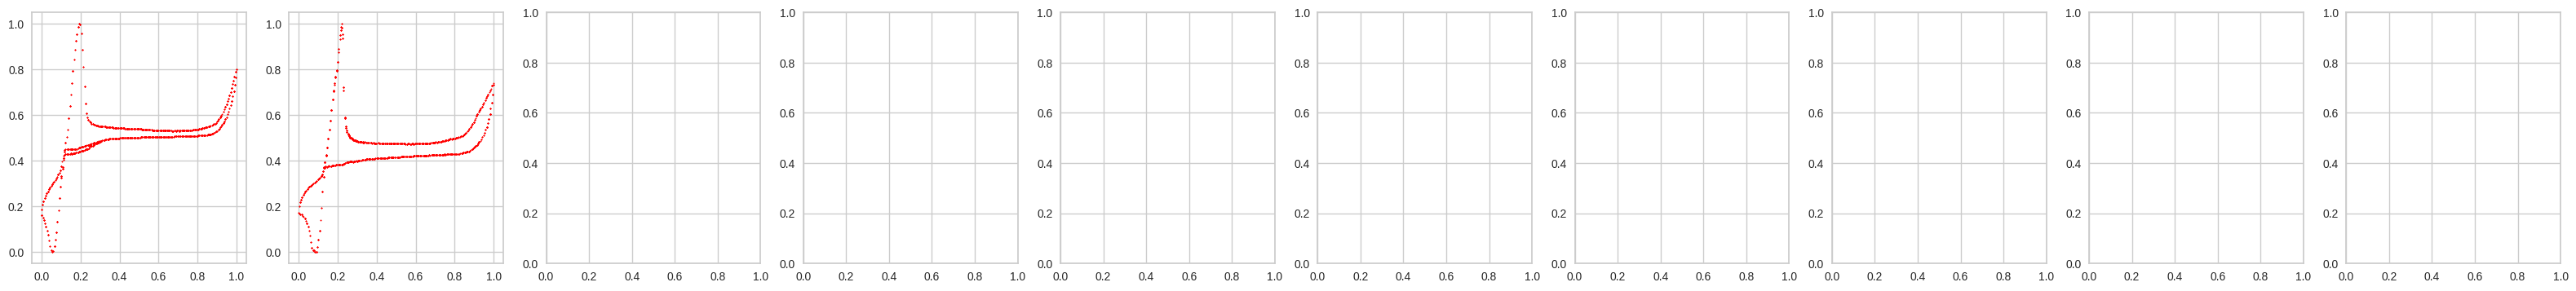
\includegraphics[width=1.0\textwidth]{figures/clusters/cv_cluster5.png}
Cluster 6:\\
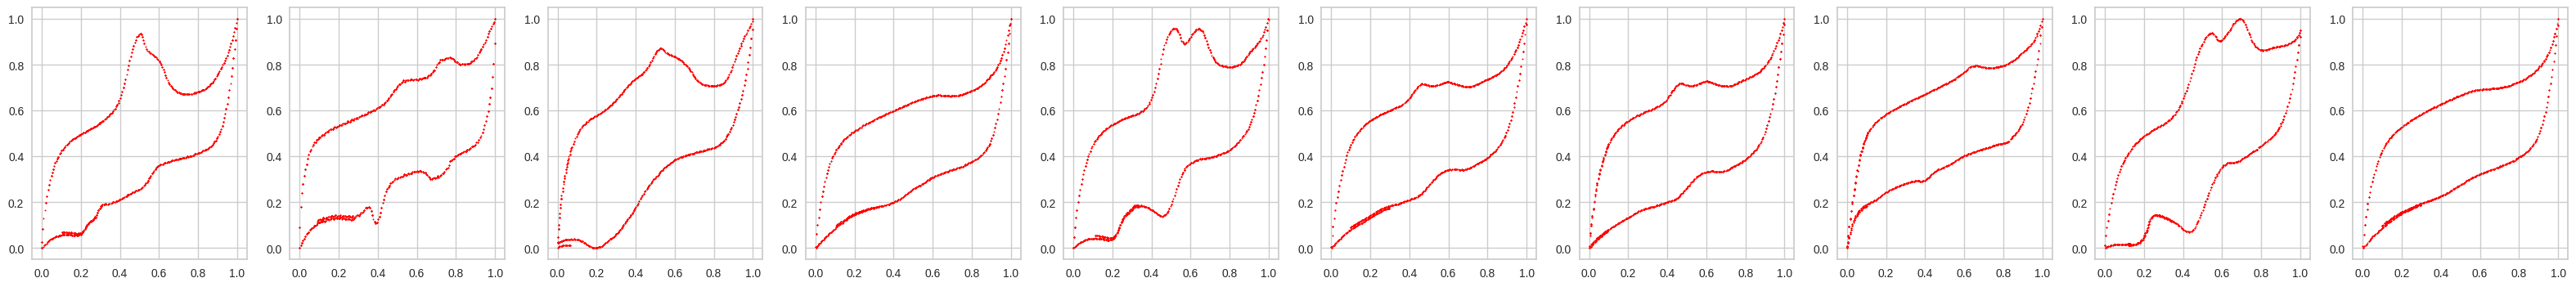
\includegraphics[width=1.0\textwidth]{figures/clusters/cv_cluster6.png}
Cluster 7:\\
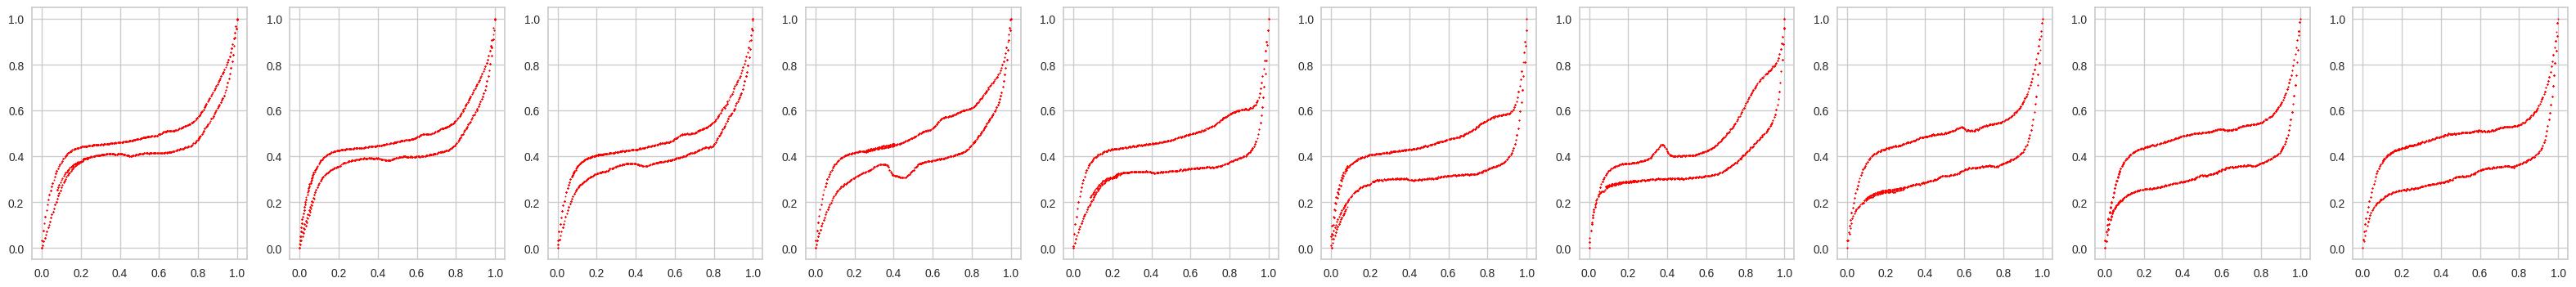
\includegraphics[width=1.0\textwidth]{figures/clusters/cv_cluster7.png}
Cluster 8:\\
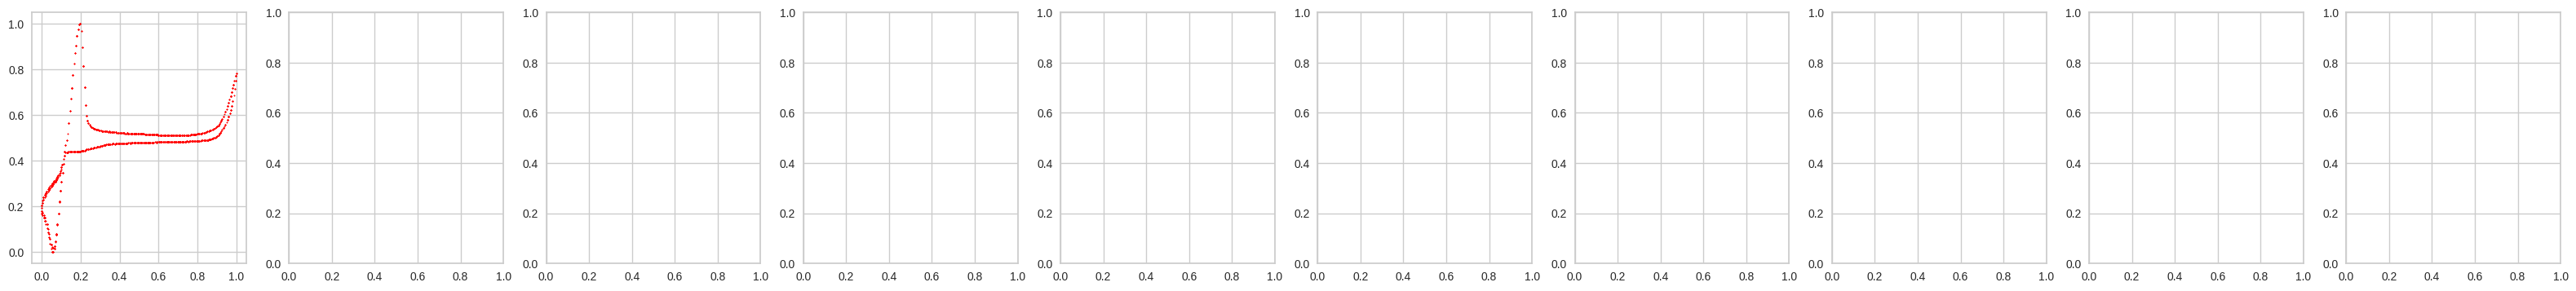
\includegraphics[width=1.0\textwidth]{figures/clusters/cv_cluster8.png}
Cluster 9:\\
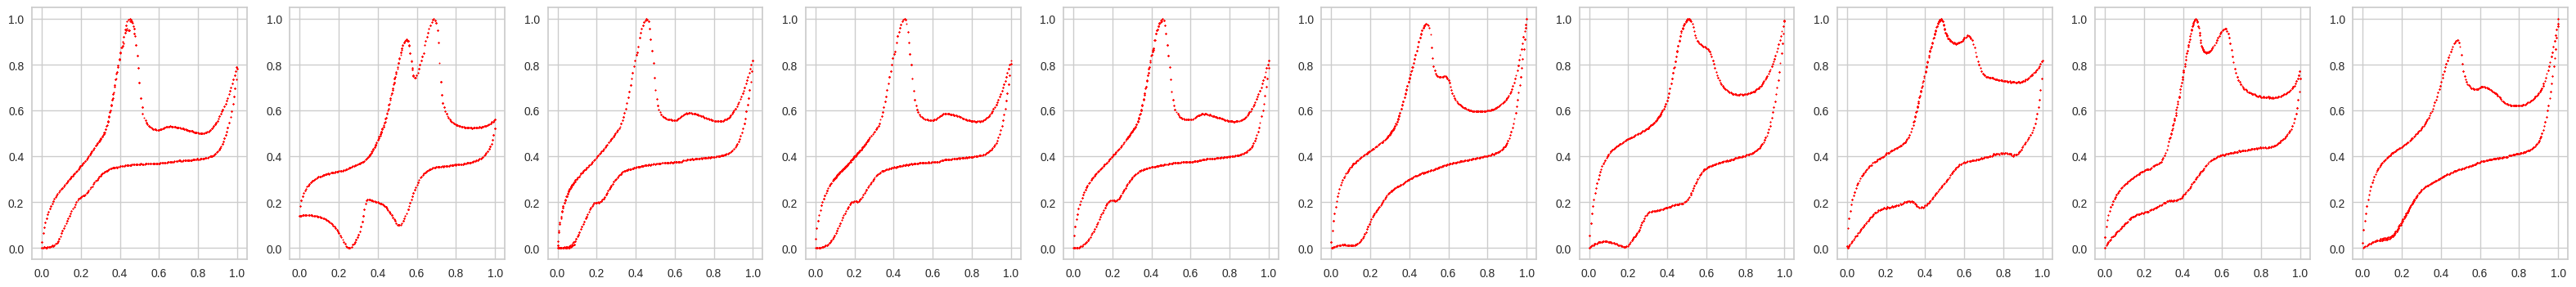
\includegraphics[width=1.0\textwidth]{figures/clusters/cv_cluster9.png}
Cluster 10:\\
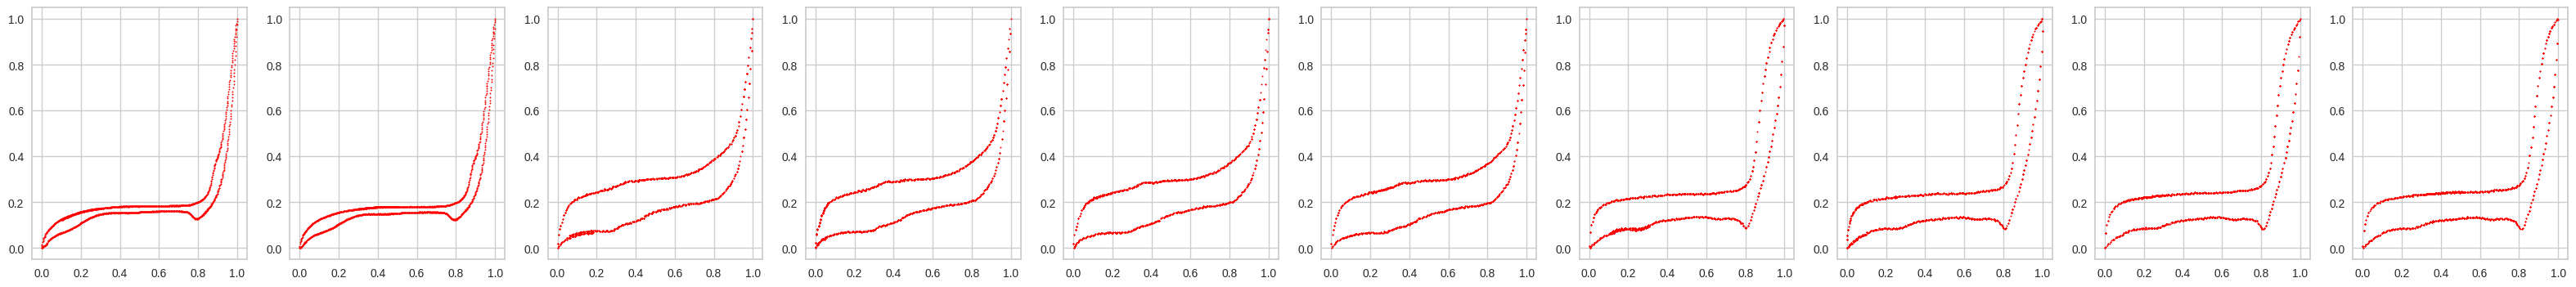
\includegraphics[width=1.0\textwidth]{figures/clusters/cv_cluster10.png}
Cluster 11:\\
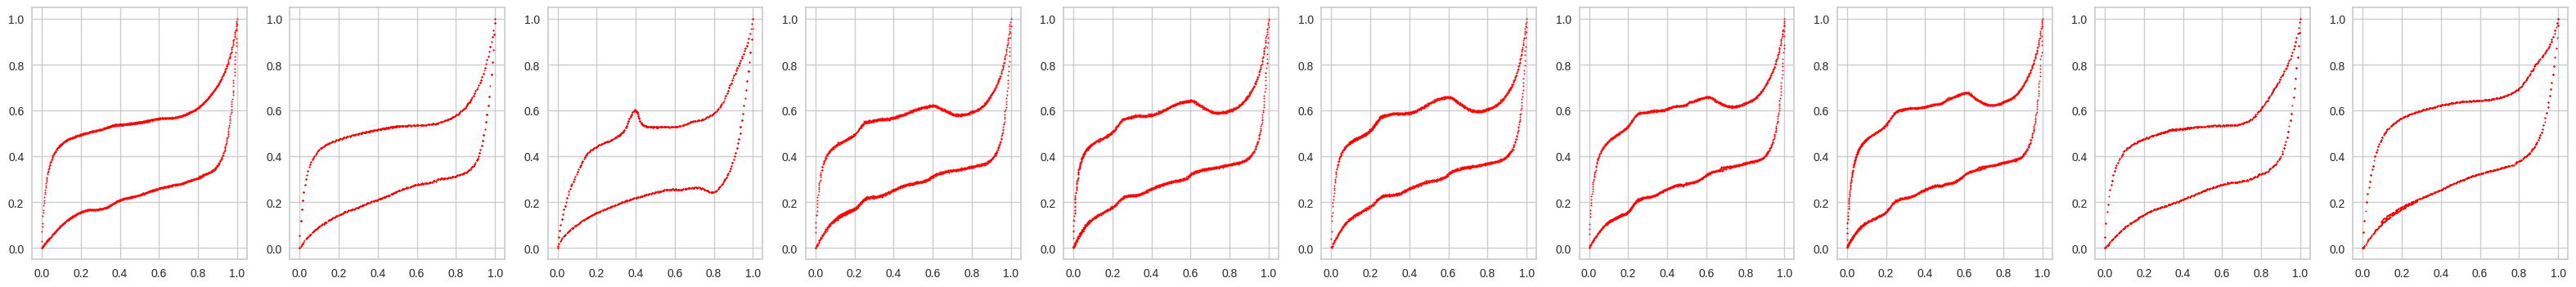
\includegraphics[width=1.0\textwidth]{figures/clusters/cv_cluster11.png}
Cluster 12:\\
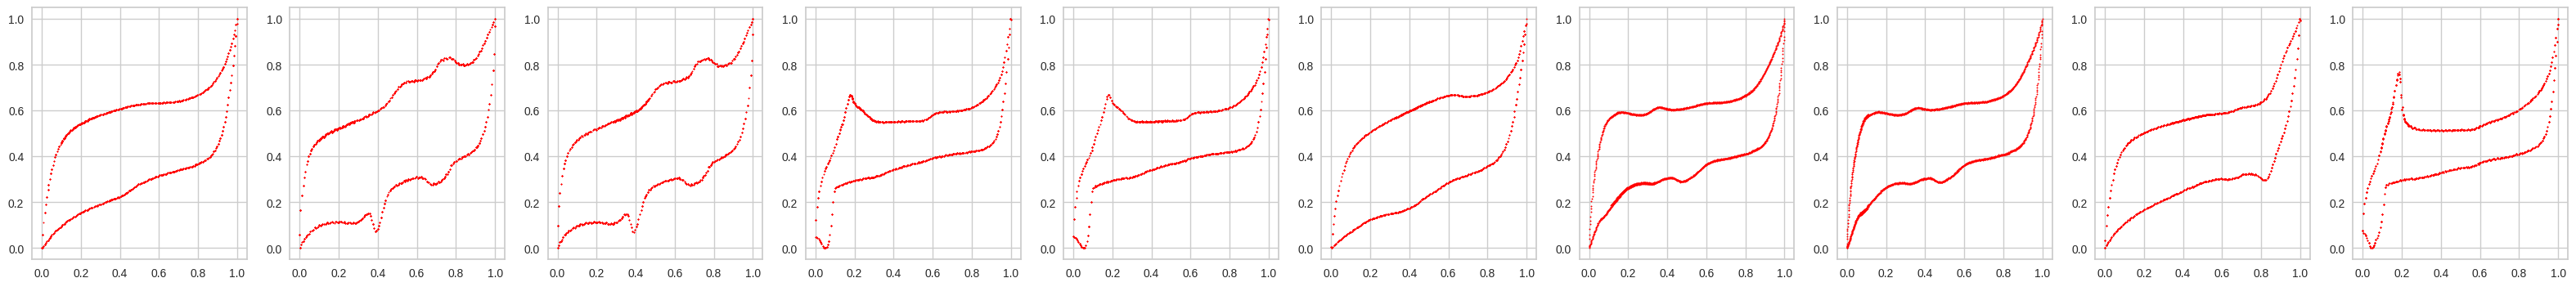
\includegraphics[width=1.0\textwidth]{figures/clusters/cv_cluster12.png}
Cluster 13:\\
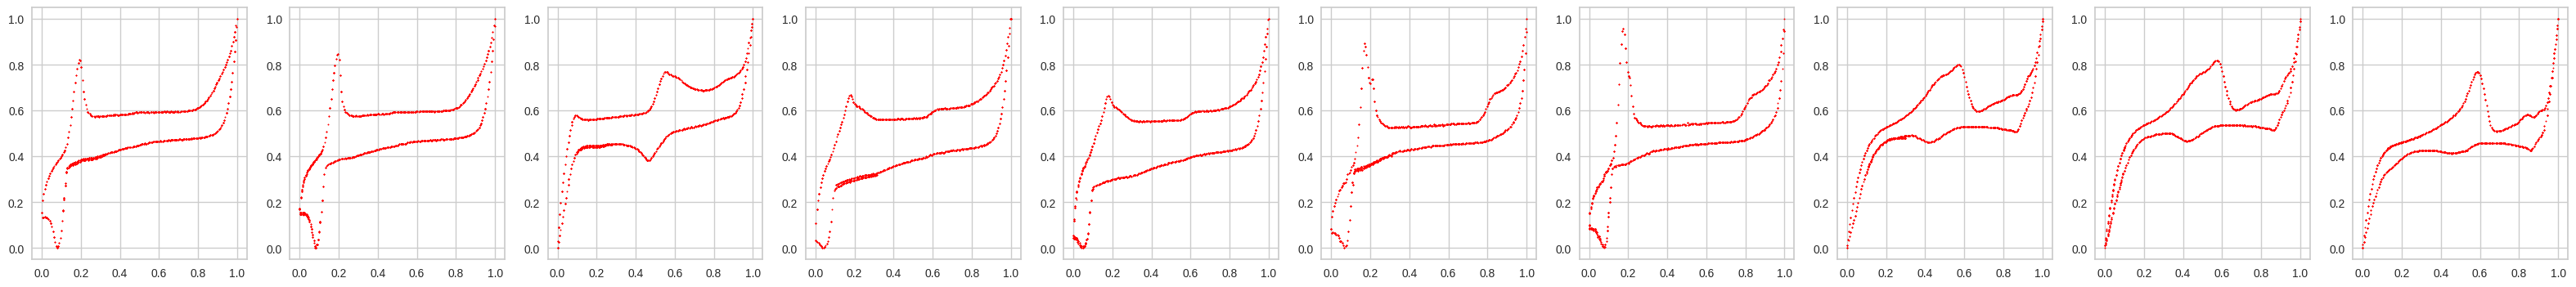
\includegraphics[width=1.0\textwidth]{figures/clusters/cv_cluster13.png}
Cluster 14:\\
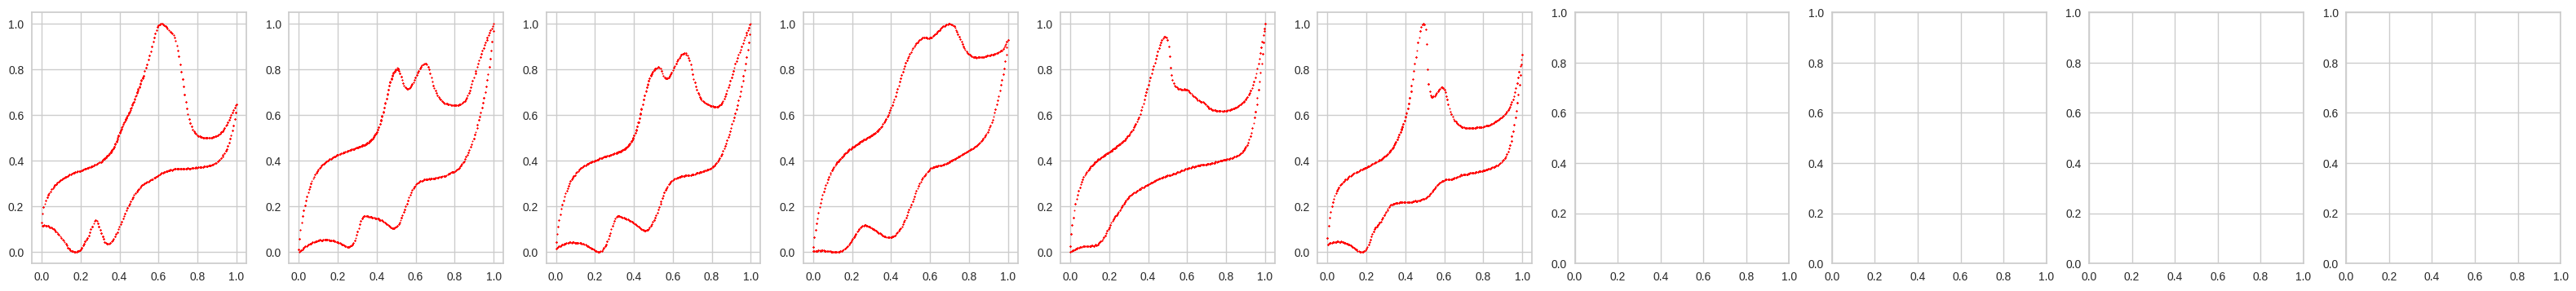
\includegraphics[width=1.0\textwidth]{figures/clusters/cv_cluster14.png}
Cluster 15:\\
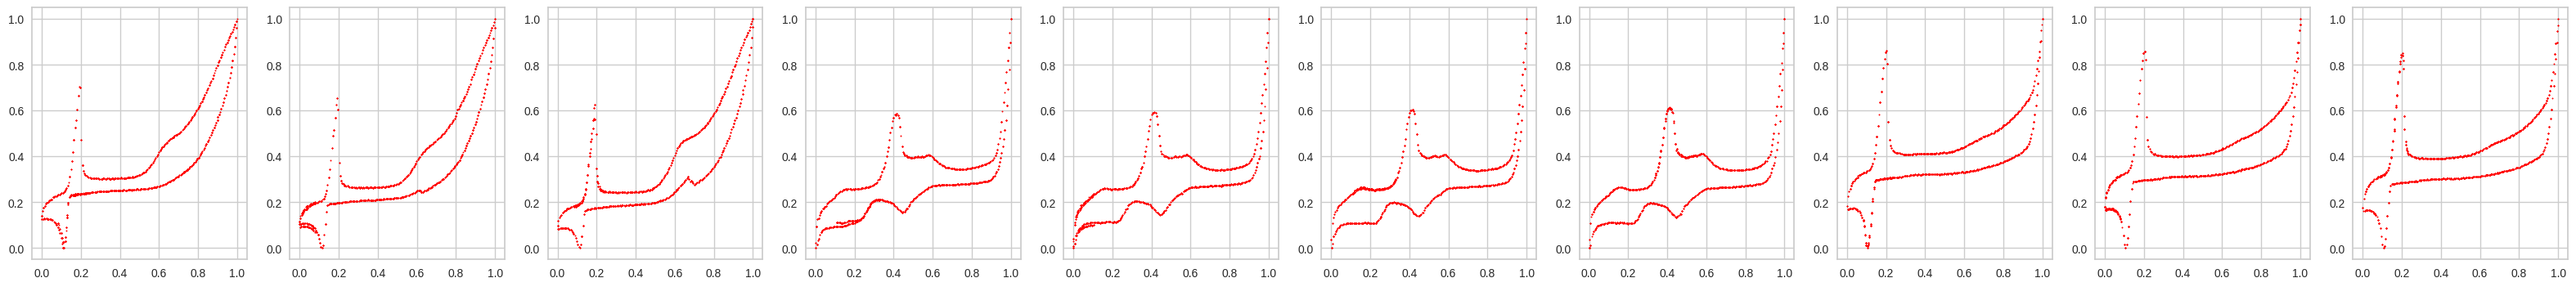
\includegraphics[width=1.0\textwidth]{figures/clusters/cv_cluster15.png}
Cluster 16:\\
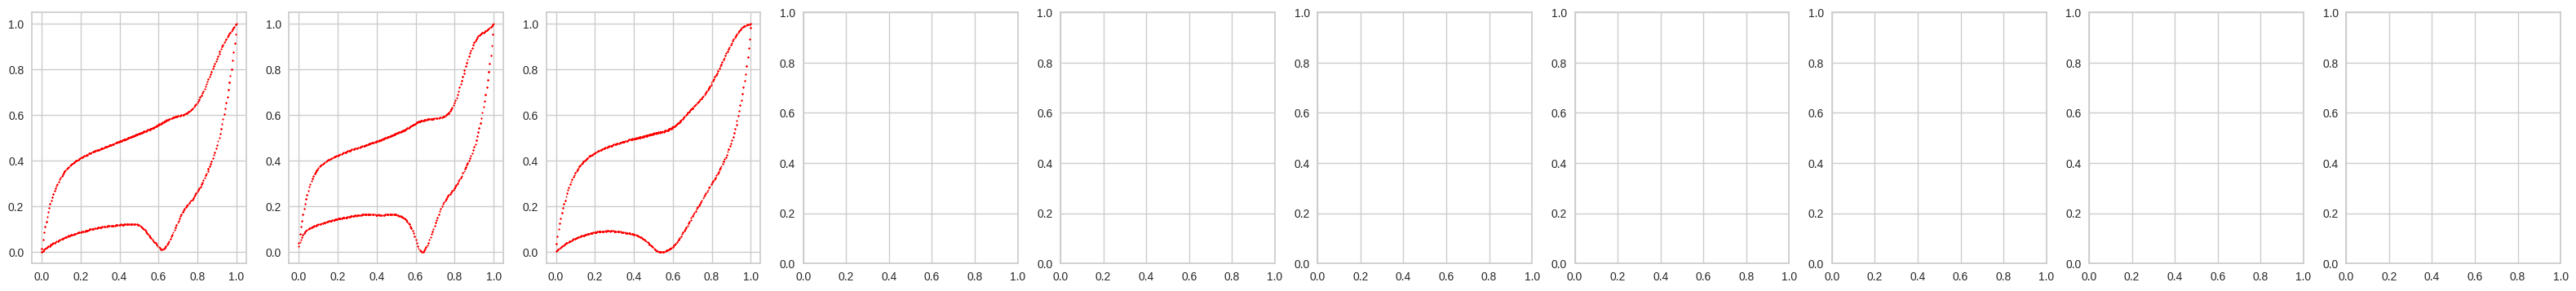
\includegraphics[width=1.0\textwidth]{figures/clusters/cv_cluster16.png}
Cluster 17:\\
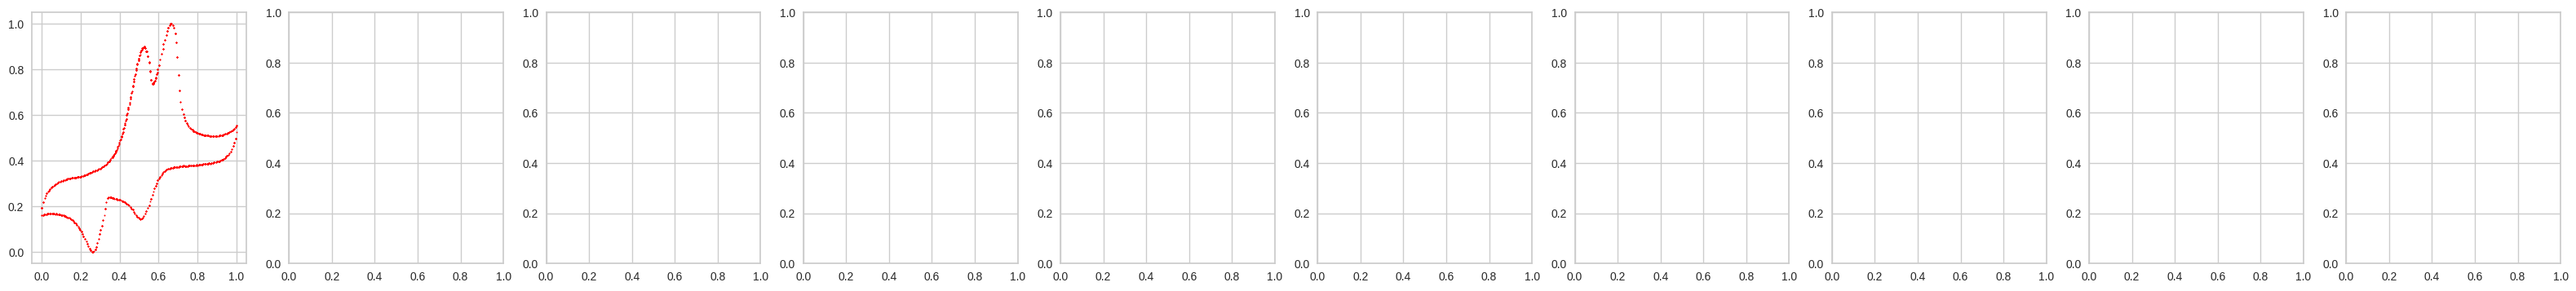
\includegraphics[width=1.0\textwidth]{figures/clusters/cv_cluster17.png}
Cluster 18:\\
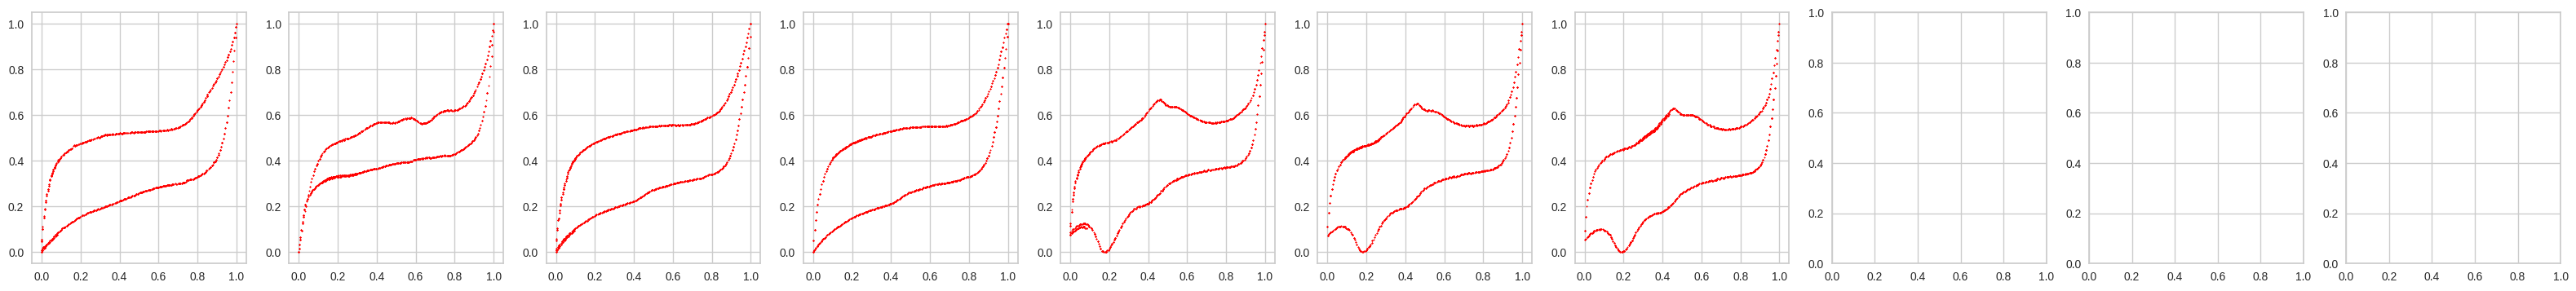
\includegraphics[width=1.0\textwidth]{figures/clusters/cv_cluster18.png}
Cluster 19:\\
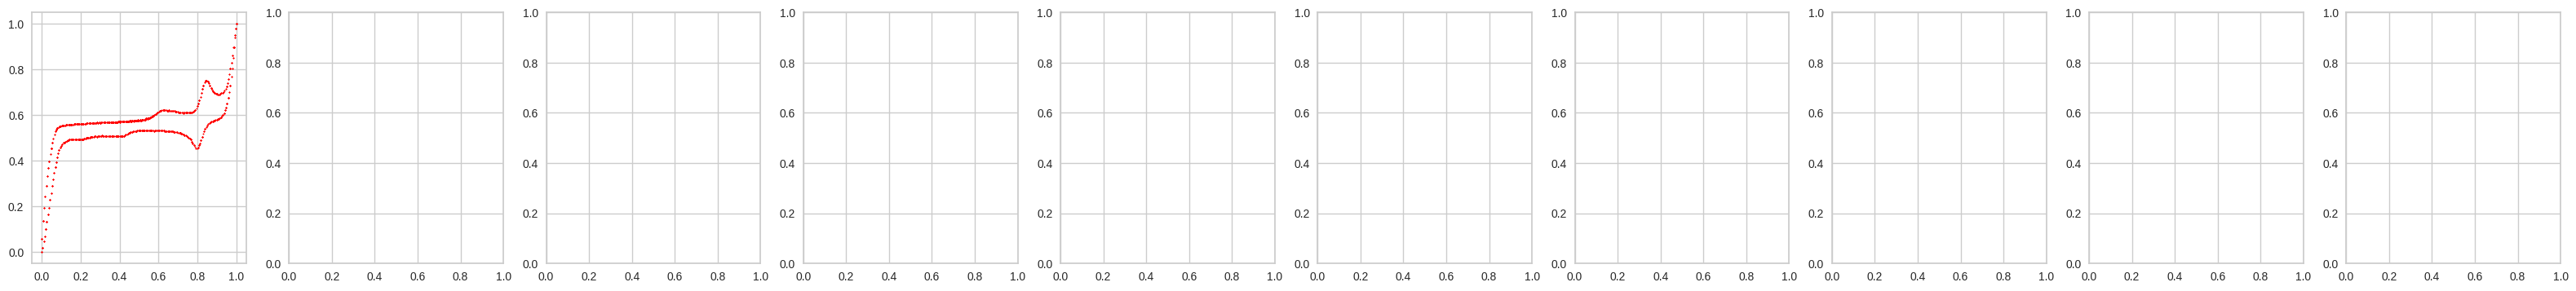
\includegraphics[width=1.0\textwidth]{figures/clusters/cv_cluster19.png}
Cluster 20:\\
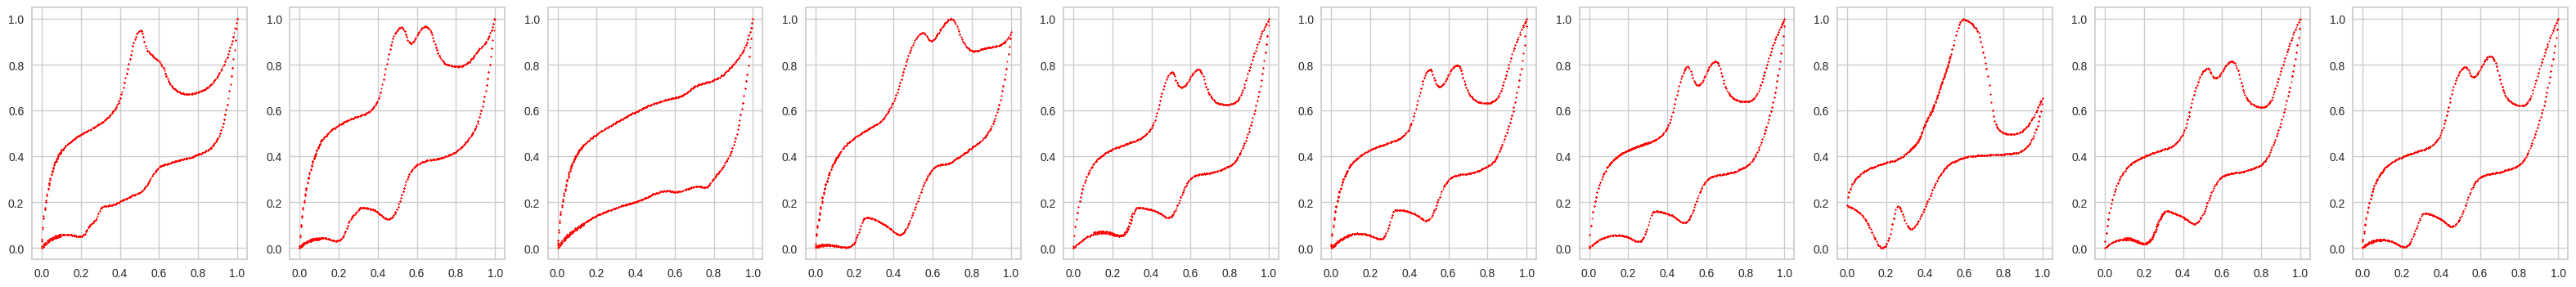
\includegraphics[width=1.0\textwidth]{figures/clusters/cv_cluster20.png}
Cluster 21:\\
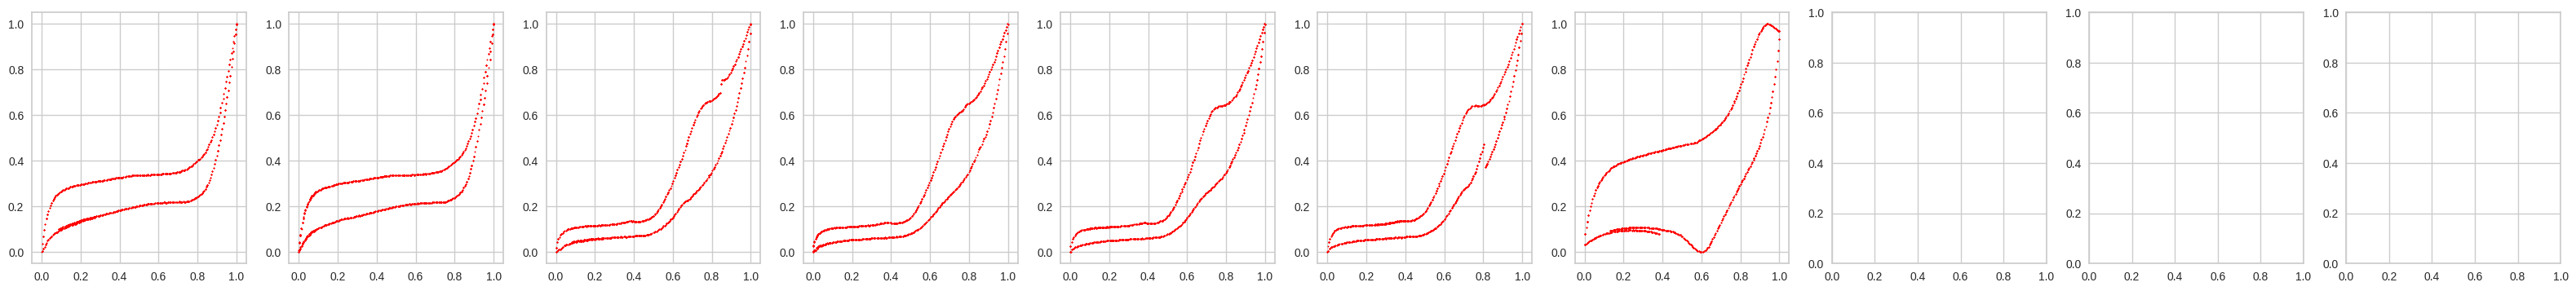
\includegraphics[width=1.0\textwidth]{figures/clusters/cv_cluster21.png}
Cluster 22:\\
\includegraphics[width=1.0\textwidth]{figures/clusters/cv_cluster22.png}
Cluster 23:\\
\includegraphics[width=1.0\textwidth]{figures/clusters/cv_cluster23.png}
Cluster 24:\\
\includegraphics[width=1.0\textwidth]{figures/clusters/cv_cluster24.png}
Cluster 25:\\
\includegraphics[width=1.0\textwidth]{figures/clusters/cv_cluster25.png}
Cluster 26:\\
\includegraphics[width=1.0\textwidth]{figures/clusters/cv_cluster26.png}
Cluster 27:\\
\includegraphics[width=1.0\textwidth]{figures/clusters/cv_cluster27.png}
Cluster 28:\\
\includegraphics[width=1.0\textwidth]{figures/clusters/cv_cluster28.png}
Cluster 29:\\
\includegraphics[width=1.0\textwidth]{figures/clusters/cv_cluster29.png}
Cluster 30:\\
\includegraphics[width=1.0\textwidth]{figures/clusters/cv_cluster30.png}
Cluster 31:\\
\includegraphics[width=1.0\textwidth]{figures/clusters/cv_cluster31.png}
Cluster 32:\\
\includegraphics[width=1.0\textwidth]{figures/clusters/cv_cluster32.png}
Cluster 33:\\
\includegraphics[width=1.0\textwidth]{figures/clusters/cv_cluster33.png}
Cluster 34:\\
\includegraphics[width=1.0\textwidth]{figures/clusters/cv_cluster34.png}
Cluster 35:\\
\includegraphics[width=1.0\textwidth]{figures/clusters/cv_cluster35.png}
Cluster 36:\\
\includegraphics[width=1.0\textwidth]{figures/clusters/cv_cluster36.png}
Cluster 37:\\
\includegraphics[width=1.0\textwidth]{figures/clusters/cv_cluster37.png}
Cluster 38:\\
\includegraphics[width=1.0\textwidth]{figures/clusters/cv_cluster38.png}

\section{Metals and Ligands}
\begin{table}[!h]
\begin{center}
\begin{tabular}{c|c|c|c}
Entry & Metal & Form & CAS \\
\hline
1 & V(IV) & $\mathrm{VOSO_4 xH_2O}$ & 123334-20-3\\
2 & Cr(III) & $\mathrm{CrK(SO_4)_2 12H_2O}$ & 7788-99-0\\
3 & Mn(II) & $\mathrm{MnSO_4H_2O}$ & 10034-96-5\\
4 & Fe(II) & $\mathrm{FeSO_47H_2O}$ & 7782-63-0\\
5 & Co(II) & $\mathrm{CoSO_47H_2O}$ & 10026-24-1\\
6 & Ni(II) & $\mathrm{NiSO_46H_2O}$ & 10101-97-0\\
7 & Cu(II) & $\mathrm{CuSO_45H_2O}$ & 7758-99-8\\
8 & Zn(II) & $\mathrm{ZnSO_47H_2O}$ & 7446-20-0\\
9 & Cd(II) & $\mathrm{CdSO_48/3H_2O}$ & 7790-84-3\\
10 & Pd(II) & $\mathrm{Na_2PdCl_4}$ & 13820-53-6\\
\end{tabular}
\caption{Table of Metals}
\label{metal_table}
\end{center}
\end{table}

\begin{table}[!h]
\begin{center}
\begin{tabular}{c|c|c|c}
Entry & Ligand & SMILES & CAS \\
\hline
1 & ammonia & N & 1336-21-6\\
2 & hydrazine & NN & 7803-57-8\\
3 & ethylenediamine & NCCN & 107-15-3\\
4 & ethanolamine & NCCO & 141-43-5\\
5 & diethanolamine & OCCNCCO & 111-42-4\\
6 & triethanolamine & OCCN(CCO)CCO & 102-71-6\\
7 & piperidine & N1CCCCC1 & 110-89-4\\
8 & morpholine & N1CCOCC1 & 110-91-8\\
9 & pyridine & n1ccccc1 & 110-86-1\\
10 & 2,2'-bipyridine (in HCl salt form) & c1ccc(nc1)c2ccccn2 & 336-18-7\\
\end{tabular}
\caption{Table of Ligands}
\label{ligand_table}
\end{center}
\end{table}

%% add more appendix chapters as you need


%% you can also add biographical sketch/ CV in here 
%% you can write it as other chapters and add the chapter in here
%% if you already have CV as a PDF, add it to the main directory, then use:

% \includepdf[pages=-]{John_Doe_CV.pdf}

%%%%%%%%%%%%%%%%%%%%%%%%%%% END BACK MATTER %%%%%%%%%%%%%%%%%%%%%%%%%%%%



\end{document}

%%%%%%%%%%%%%%%%%%%%%%%%% DOCUMENT ENDS HERE %%%%%%%%%%%%%%%%%%%%%%%%%%%